\documentclass[11pt]{article}

\usepackage{xcolor}
\definecolor{darkpastelgreen}{rgb}{0.01, 0.75, 0.24}

\usepackage[colorlinks=true,
            linkcolor=red,
            urlcolor=darkpastelgreen,
            citecolor=blue,
            breaklinks=true]{hyperref}
\usepackage{breakurl} 
\usepackage[a4paper, left=3cm, right=3cm, top=3cm, bottom=3cm]{geometry}
\RequirePackage{amsmath,amsfonts, amssymb,amsthm}

\hypersetup{pdfauthor = {Simon Bussy}}

\usepackage{authblk}
\title{\vspace{-.5cm} Lights: a generalized joint model for high-dimensional multivariate longitudinal data and censored durations \vspace{.5cm}}
\author[1,2]{Simon Bussy\thanks{Corresponding author: \href{mailto:simon.bussy@gmail.com}{\texttt{simon.bussy@gmail.com}}}}
\author[2]{Van Tuan Nguyen}
\author[3]{Antoine Barbieri}
\author[1]{Sarah Zohar}
\author[1,4]{Anne-Sophie Jannot}
\affil[1]{INSERM, UMRS 1138, Centre de Recherche des Cordeliers, Paris, France}
\affil[2]{Califrais' Machine Learning Lab, Paris, France}
\affil[3]{INSERM, UMR 1219, Bordeaux Population Health Research Center, Univ. Bordeaux, France}
\affil[4]{Biomedical Informatics and Public Health Department, EGPH, APHP, Paris, France}
\setcounter{Maxaffil}{0}
\renewcommand\Affilfont{\itshape\small}

\usepackage{mathtools}
\usepackage{mathrsfs}
\usepackage{mathrsfs} 
\usepackage{natbib}
\usepackage{setspace}
\usepackage{dsfont}
\usepackage{caption}
\usepackage{booktabs}
\usepackage{subfigure}
\usepackage{algpseudocode}
\usepackage[linesnumbered,ruled,vlined]{algorithm2e}
\newcommand\mycommfont[1]{\footnotesize\ttfamily\textcolor{orange}{#1}}
\SetCommentSty{mycommfont}
\SetKwInput{KwInput}{Input} 
\SetKwInput{KwOutput}{Output}

\newtheorem{assumption}{Assumption}{\bf}{\rm} 
\newtheorem{lemma}{Lemma}

\DeclareMathOperator{\argmin}{argmin}
\DeclareMathOperator{\Tr}{Tr}

\newcommand{\dd}{\mathrm{d}}
\newcommand{\ind}[1]{\mathds{1}_{#1}}
\newcommand{\norm}[1]{\|#1\|}
\newcommand{\cM}{\mathcal M}
\newcommand{\cD}{\mathcal D}
\newcommand{\cC}{\mathcal C}
\newcommand{\cG}{\mathcal G}
\newcommand{\cN}{\mathcal N}
\newcommand{\cA}{\mathcal A}
\newcommand{\cQ}{\mathcal Q}
\newcommand{\cU}{\mathcal U}
\newcommand{\cR}{\mathcal R}
\newcommand{\cH}{\mathcal H}
\newcommand{\cB}{\mathcal B}
\newcommand{\cS}{\mathcal S}
\newcommand{\R}{\mathds R}
\newcommand{\N}{\mathds N}
\newcommand{\E}{\mathds E}
\renewcommand{\P}{\mathds P}
\newcommand{\bSigma}{\textbf{$\Sigma$}}

\date{}

\begin{document}

\maketitle

\vspace{-.5cm}

\begin{abstract}

This paper introduces a prognostic method called \textit{lights} to deal with the problem of joint modeling of longitudinal data and censored durations, where a large number of longitudinal features are available. Yet there is no standard model so far to learn from such high-dimensional multivariate longitudinal data in a survival analysis setting.
Features are extracted from the longitudinal processes and included as potential risk factor in a group-specific Cox model with high-dimensional shared associations. Appropriate penalties are then used during inference to allow flexibility in modeling the dependency between the longitudinal features and the event time.
The statistical performance of the method is examined on an extensive Monte Carlo simulation study, and finally illustrated on publicly available datasets.
On these high-dimensional datasets, our proposed method significantly outperforms the state-of-the-art survival models regarding risk prediction in terms of C-index, with a computing time orders of magnitude faster. In addition, it provides powerful interpretability by automatically pinpointing significant features being relevant from a practical perspective. Thus, we propose a powerfull tool with the ability of automatically determining significant prognostic longitudinal features, which is of increasing importance in many areas: for instance personalized medicine, or churn prediction in a customer profile and activity monitoring setting, to name but a few.\\

\noindent
\emph{Keywords.} High-dimensional estimation; Joint modeling; Multivariate longitudinal data; Survival analysis
\end{abstract}

\section{Introduction}

With the increasing expectations to know their customers from account opening throughout the duration of the business relationship, web companies have the luxury of building elaborate systems to help them keep everything on track. The amount of recorded data per client is often tremendous and growing through time. There is no tool today to take into account simultaneously a huge number of longitudinal signals in a high-dimensional context to perform real-time churn (or satisfaction) risk prediction.
Similarly, in many clinical studies, it has become increasingly common to record the values of longitudinal features (e.g., biomarkers) until the occurrence of an event of interest for a subject. The ``joint modeling'' approaches, namely modeling the longitudinal and survival outcomes through a joint likelihood model rather than separately, has received considerable attention during the past two decades~\citep{tsiatis2004joint}. Numerical studies suggest that these approaches are among the most satisfactory to combine information~\citep{yu2004joint}. They have the advantage of making more efficient use of the data since information about survival also goes into modeling the longitudinal features. In addition, they produce unbiased estimates and do not rely on approximations for incorporating conplex longitudinal trajectories. Most developments have either focused on shared random-effect models (SREMs)~\citep{wulfsohn1997joint}, in which characteristics of the longitudinal processes (for instance functions of the random effects) are included as features in the survival model ; or on joint latent class models (JLCMs)~\citep{vermunt2003latent}, in which the population is considered as heterogeneous, with the assumption that there exist homogeneous latent subgroups sharing the same marker trajectories and the same prognostic.

\paragraph{The high-dimensional longitudinal data context.}
With the exploding number of daily internet users, or with the development of electronic health records in a medical context, high-dimensional settings are becoming increasingly frequent in various contexts where the number of available features to consider as potential risk factors is tremendous.
Moreover, with an increased focus on personalised medicine, the need to implement multivariate models that account for a large number of longitudinal outcomes is critical. Despite this, joint models have predominantly focused on univariate data, with attempts to fit multiple univariate joint models separately~\citep{wang2012joint}, which is inefficient~\citep{lin2002maximum}. 
Despite many multivariate models being presented in full generality, questions arrising from the high-dimensional context -- e.g., computational power, limits in numerical estimation, or sample size -- are never considered in analyses (to the best of our knowledge), and the number of longitudinal outcomes considered in numerical studies are often very low (see~\citet{hickey2016joint} for a complete review). For instance,~\citet{jaffa2014joint} only considers 3 longitudinal outcomes in the simulation study while mentioning a ``high-dimensional multivariate longitudinal data'' context.


\paragraph{General framework.}

The setting of this paper is such that we want to incorporate high-dimensional time-dependent (longitudinal) features measured with error in a survival model. Let us consider the usual survival analysis framework.
Following~\citet{andersen2012statistical}, let non-negative random variables $T^\star$ and $C$ stand for the times of the event of interest and censoring times respectively. The event of interest could be for instance survival time, re-hospitalization, relapse or disease progression in a medical context; or the time when a client stops using a company's product or service in a churn prediction setting.
We then denote $T$ the right-censored time and $\Delta$ the censoring indicator, defined as 
\begin{equation*}
T = T^\star \wedge C \quad \text{and} \quad \Delta = \ind{\{T^\star \leq C\}}
\end{equation*}
respectively, where $a \wedge b$ denotes the minimum between two numbers $a$ and $b$, and $\ind{\{\cdot\}}$ the indicator function taking the value $1$ if the condition in $\{\cdot\}$ is satisfied and $0$ otherwise.

Let $X$ denotes the $p$-dimensional vector of time-independent features (e.g., patients characteristics, therapeutic strategy, or omics features recorded at the begining of a medical study), and let  $Y(t) = \big(Y^1(t), \ldots, Y^L(t) \big)^\top \in \R^L$ denote the value of the $L$-dimensional longitudinal outcome at time point $t \geq 0$, with $L \in \N_+$.


\paragraph{Heterogeneity of the population.}

An assumption of heterogeneity within the subject population is frequently relevant in medical research where several differing profiles of subjects are expected~\citep{bussy2019c}. To take account of this, we introduce a latent variable $G \in \{0, \ldots, K-1\}$ modeling the $K \geq 1$ subgroups of different risk, which is a classical modeling assumption in JLCMs~\citep{lin2002latent, proust2014joint}. Let us denote
\begin{equation}
  \label{eq:pi}
  \pi_{\xi_k}(x) = \P[G=k|X=x]
\end{equation}
the latent class membership probability given time-independent features $x \in \R^p$, and consider a softmax link function given by
\begin{equation}
  \label{eq:pi-softmax} 
  \pi_{\xi_k}(x) = \dfrac{e^{x^\top\xi_k}}{\sum_{k=0}^{K-1}e^{x^\top\xi_k}}
\end{equation}
where $\xi_k \in \R^p$ denotes a vector of coefficients that quantifies the impact of each time-independent features on the probability that a subject belongs to the $k$-th group, with $\xi_0 = \mathbf{0}_p$ for overparameterization purpose, where $\mathbf{0}_p$ stands for the vector of $\R^p$ having all coordinates equal to zero. The intercept term is here omitted without loss of generality. 
From now on, all computations are done conditionally on features $x$.

\paragraph{Main contribution.} 

In this paper, we propose a method called \textit{lights} (generaLized joInt hiGH-dimensional longiTudinal Survival) which is from both JLCMs and SREMs, since we also include features extracted from the longitudinal processes as potential risk factor in the survival model, which is a group-specific Cox model~\citep{Cox1972JRSS} with high-dimensional shared associations.
To allow flexibility in modeling the dependency between the longitudinal features and the event time, we use appropriate penalties : elastic net~\citep{zou2005regularization}
for feature selection in the latent class membership, and sparse group lasso~\citep{simon2013sparse} in the survival model, as well as for the fixed effect (allowing flexible representations of time). Indeed, this penalty acts like the lasso at the trajectory level, namely an entire trajectory may drop out of the model on one side. On the other hand, it yields sparsity for a given trajectory, namely feature selection.
Inference is achieved using an efficient and novel Quasi-Newton Monte Carlo Expectation Maximization algorithm.
Posterior estimates of the latent class membership probabilities given the longitudinal process and the fact that the subject is still alive at prediction time -- in a so called ``real-time prediction paradigm'' -- are then used as discriminative marker rule for risk prediction in the cross-validation procedure for selecting the best regularization hyper-parameters (to perform feature selection and adapt to the longitudinal data complexity).
Hence, the method provides interpretations of the high-dimensional longitudinal features, thus offering a powerful tool for clinical decision making in patient monitoring for instance, or else for real-time decision support in a customer's satisfaction monitoring context.

\paragraph{Organization of the paper.}

A precise description of the model is given in Section~\ref{sec:Method}.
Section~\ref{sec:inference} focuses on a regularized version of the
model to exploit dimension reduction and prevent overfitting. Inference is
presented under this framework, as well as the developed algorithm.
Section~\ref{sec:Performance evaluation} introduces the C-index metric, as well as a novel evaluation strategy to assess diagnostic prediction performances while mimicking a real-time use of the model in clinical care, and finally the considered competing methods.
Section~\ref{sec:simulation study} presents the simulation procedure used to evaluate the performance of our method in a high-dimensional context and compares it with state-of-the-art ones. In Section~\ref{sec:application}, we apply our method to high-dimensional publicly available datasets. Finally, we discuss the obtained results in Section~\ref{sec:conclusion}.

\paragraph{Notations.}

Throughout the paper, for every $q > 0,$ we denote by $\norm{v}_q$ the usual $\ell_q$-quasi norm of a vector $v \in \R^m,$ namely $\norm{v}_q =(\sum_{k=1}^m|v_k|^q)^{1/q}$. We also denote $\norm{v}_0 = |\{k : v_k \neq 0\}|$, where $|A|$ stands for the cardinality of a finite set $A$. $\lfloor a \rfloor$ denotes the largest integer less than or equal to $a \in \R$.
For $u, v \in \R^m$, we denote by $u \odot v$ the Hadamard product $u\odot v =(u_1v_1, \ldots, u_mv_m)^\top.$ 
For a squared matrix $M$, $\text{vech}(M)$ stacks columns of $M$ one under another in a single vector, starting each column at its diagonal element. We write $I_m$ for the identity matrix of $\R^{m \times m}$.
Finally, we write, for short, $\mathbf{1}_m$  (resp. $\mathbf{0}_m$) for the vector of $\R^m$ having all coordinates equal to one (resp. zero).


\section{Method}
\label{sec:Method}

In this section, we descibe the longitudinal and time-to-event submodels, as well as the required hypothesis in order to write a likelihood and draw inference for the lights model.

\subsection{Group-specific marker trajectories}

We suppose a group-specific marker trajectory and a generalized linear mixed model for each longitudinal marker given subgroup $G$, so that for the $l$-th outcome at time $t \geq 0$ one has
\begin{equation}
	\label{eq:link-function}
 	h_l\big(\E[Y^l(t)|b^l, G=k]\big) = m_k^l(t)
 \end{equation}
where $h_l$ denotes a known one-to-one link function, and $m_k^l$ the linear predictor such that
\[ m_k^l(t) = u^l(t)^\top\beta_k^l + v^l(t)^\top b^l \]
where $u^l(t) \in \R^{q_l}$ is a row vector of (possibly) time-varying features with corresponding unknown fixed effect parameters $\beta_k^l$, and $v^l(t) \in \R^{r_l}$ is a row vector of (possibly) time-varying features with $r_l \leq q_l$ and where the corresponding subject-and-longitudinal outcome specific random effects $b^l$ that does not depend on the group membership, which is not a strong modeling assumption.
\begin{assumption}
\label{assumption1}
We suppose that the random effects are independent of the group membership, and that the latter remain independent conditional on the observed data (namely $T$, $\Delta$ and $Y$).
\end{assumption}
A suitable distributional assumption for the random effects component is a zero-mean multivariate normal distribution~\citep{hickey2016joint}, that is
\begin{equation}
   \label{eq:random-effect-law}
   b^l \sim \cN(0, D_{ll})
 \end{equation} 
with $D_{ll} \in \R^{r_l \times r_l}$ the unstructured variance-covariance matrix. 
To account for dependence between the different longitudinal outcome types, we let $\text{Cov}[b^l,b^{l'}] = D_{ll'}$ for $l \ne l'$ and we denote
\[ D = 
\begin{bmatrix}
  D_{11} & \cdots & D_{1L}\\
  \vdots &  \ddots & \vdots \\
  D_{1L}^\top & \cdots & D_{LL}
\end{bmatrix}
\]
the global variance-covariance matrix.
In the sequel of the paper, our aim is to associate the true and unobserved value $m_k^l(t)$ of the $l$-th longitudinal outcome at time $t$ with the event outcome $T^\star$.

\subsection{Group-specific risk of event}

To quantify the effect of the longitudinal outcomes on the risk for an event, we use a Cox~\citep{Cox1972JRSS} relative risk model of the form
\begin{equation}
	\label{eq:intensity-model}
	\lambda(t|\cM_k(t), G = k) = \lambda_0(t) \exp \Big\{ x^\top \gamma_k^0 + \sum_{l=1}^L \sum_{a=1}^\cA {\gamma_{k,a}^l}^\top \varphi_a(t, \beta_k^l, b^l) \Big\},
\end{equation}
where $\lambda_0(\cdot)$ is an unspecified baseline hazard function and given that $G = k$, we denote 
\[\cM_k(t) = \{m_k^l(u), 0 \leq u < t\}\] 
the history of the true unobserved longitudinal process up to time $t$. We choose to incorporate $x$, also used in~\eqref{eq:pi}, with no \textit{a priori} on the choice of time-independent features involved in the definition of $\pi_{\xi_k}$ nor $\lambda$, since independent regularizations are used during inference, see~\eqref{eq:pen-log-lik}. Corresponding fixed effects are denoted $\gamma_k^0 \in \R^p$, and for each $l$-th longitudinal outcome, we consider $\cA \in \N_+$ known functionals $\varphi_a$ defining a shared association with $\gamma_{k,a}^l \in \R^{\imath_a}$ the corresponding joint association parameters, and $\imath_a \in \N_+$ the dimension of the corresponding $\text{Im}(\varphi_a)$. 
This can be viewed as a generalization of SREMs~\citep{rizopoulos2010jm}. Let us finally denote
\[({\gamma_k^0}^\top, \gamma_k^\top)^\top= ({\gamma_k^0}^\top, \gamma_{k,1}^1, \ldots, \gamma_{k,\cA}^1, \ldots, \gamma_{k,1}^L, \ldots, \gamma_{k,\cA}^L )^\top \in \R^{p+L\cA}. \]

\paragraph{Specification of the functionals $(\varphi_a)_{a\in \cA}$.}

The association structure between the longitudinal and the time-to-event submodels is key to the joint modeling framework. In spite of that, rationale for selecting shared associations has received little attention. We then propose to include some of the most common parameterization with no \textit{a priori}, set out in Table~\ref{table:shared_associations}, and let the model select the relevant ones through the regularization strategy described in Section~\ref{sec:penalized-obj}.
\begin{table}[htb]
\centering
\begin{tabular}{ccccc}
\toprule
Description & $\varphi_a(t, \beta_k^l, b^l)$ & $\frac{\partial \varphi_a(t, \beta_k^l, b^l)}{\partial \beta_k^l}$ & $\imath_a$ & Reference \\
\midrule
Linear predictor & $m_k^l(t)$ & $u^l(t)$ & 1 & \citet{chi2006joint} \\ [.15cm]
Random effects & $b^l$ & $\mathbf{0}_{q_l}$ & $r_l$ & \citet{hatfield2011joint} \\ 
Time-dependent slope & $\dfrac{\dd}{\dd t} m_k^l(t)$ & $\dfrac{\dd}{\dd t} u^l(t)$ & 1 & \citet{rizopoulos2011bayesian} \\ [.3cm]
Cumulative effect & $\int_0^t m_k^l(s) \dd s$ & $\int_0^t u^l(s) \dd s$ & 1 & \citet{andrinopoulou2017combined} \\ [.1cm]
 \bottomrule
\end{tabular}
\caption[]{Description of the shared associations included in the group-specific risk of event submodel~\eqref{eq:intensity-model}. The gradient with respect to $\beta_k^l$ is also given, which will be useful for inference in Section~\ref{sec:QNMCEM}.}
\label{table:shared_associations}
\end{table}
 
\subsection{Likelihood}

Consider an independent and identically distributed (i.i.d.) cohort of $n$ subjects
\[ \cD_n = \big\{ (x_1, y_1^1, \ldots, y_1^L, t_1, \delta_1), \ldots, (x_n, y_n^1, \ldots, y_n^L, t_n, \delta_n) \big\} \]
where for each subject $i=1, \ldots, n$, process $Y_i^l$ is measured $n_i^l$ times at $t_{i1}^l, \ldots, t_{in_i^l}^l$ (which can differ between subjects and outcomes) with $t_{ij}^l \leq t_{ij+1}^l$ for all $j=1, \ldots, n_i^l-1$ and such that
\[ y_i^l=(y_{i1}^l, \ldots, y_{in_i^l}^l)^\top \in \R^{n_i^l} \quad \text{ with } \quad y_{ij}^l=Y_i^l(t_{ij}^l) \]
for all $l=1, \ldots, L$. 
For the $i$-th subject, let us denote 
\[
\left\{
    \begin{array}{ll}
        y_i &= ({y_i^1}^\top \cdots {y_i^L}^\top)^\top \in \R^{n_i},\\
        b_i &= ({b_i^1}^\top \cdots {b_i^L}^\top)^\top \in \R^r,
    \end{array}
\right.
\]
with $n_i = \sum_{l=1}^L n_i^l$ and $r = \sum_{l=1}^L r_l$ the total number of longitudinal measurements (for subject $i$) and the total dimension of the random effects respectively, as well as the following design matrices
\[ U_i = 
\begin{bmatrix}
  U_{i1} & \cdots & 0\\
  \vdots &  \ddots & \vdots \\
  0 & \cdots & U_{iL}
\end{bmatrix} 
\in \R^{n_i \times q}
\qquad \text{and} \qquad
V_i = 
\begin{bmatrix}
  V_{i1} & \cdots & 0\\
  \vdots &  \ddots & \vdots \\
  0 & \cdots & V_{iL}
\end{bmatrix}
\in \R^{n_i \times r}
\]
with $q = \sum_{l=1}^L q_l$ and where for all $l=1, \ldots, L$, one writes
\[
\left\{
    \begin{array}{ll}
        U_{il} &= \big(u_i^l(t_{i1}^l)^\top \cdots u_i^l(t_{in_i^l}^l)^\top\big)^\top \in \R^{n_i^l \times q_l},\\
        V_{il} &= \big(v_i^l(t_{i1}^l)^\top \cdots v_i^l(t_{in_i^l}^l)^\top\big)^\top \in \R^{n_i^l \times r_l}.
    \end{array}
\right.
\]
From now on, all computations are done conditionally on the design matrices $(U_i)_{i=1, \dots, n}$ and $(V_i)_{i=1, \dots, n}$.
\begin{assumption}
\label{indep-hyp-2}
Suppose that for a given subject $i$ and conditional on the random effects and the group membership, all $Y_i^l$ are independent for $l=1, \dots, L$.
\end{assumption}
Assumption~\ref{indep-hyp-2} is similar to standard modeling hypothesis, see for instance~\citet{tsiatis2004joint}.
For all $k = 0, \ldots, K-1$, we denote 
\[ \beta_k = ({\beta_k^1}^\top \cdots {\beta_k^L}^\top)^\top \in \R^q \] 
and 
\[M_{ik} = U_i\beta_k + V_ib_i \in \R^{n_i}. \]

Given~\eqref{eq:link-function} and Assumption~\ref{indep-hyp-2}, each $y_i^l$ is assumed to be from a one-parameter exponential family with respect to a reference measure which is either the Lebesgue measure (e.g., in the Gaussian case) or the counting measure (e.g., in the logistic cases).
The conditional distribution of $y_i|b_i, G_i=k$ is then assumed to be from a distribution with a density of the form
\begin{equation}
	\label{eq:exp-family-density}
	f(y_i|b_i, G_i=k) = \exp \big\{(y_i \odot \Phi_i)^\top M_{ik} - c_\phi(M_{ik}) + d_\phi(y_i) \big\},
\end{equation}
with 
\[ \Phi_i = (\phi_1^{-1} {\textbf{1}_{n_i^1}}^\top \cdots \phi_L^{-1} {\textbf{1}_{n_i^L}}^\top)^\top \in \R^{n_i} \] 
and $\phi = (\phi_1, \ldots, \phi_L)^\top \in \R^L$.
The density described in~\eqref{eq:exp-family-density} encompasses several distributions, see Table~\ref{table:glm}. The functions $c_\phi(\cdot)$ and $d_\phi(\cdot)$ are known as well as the dispersion parameters $\phi_l$, while parameters $\beta_k$ have to be estimated. Note that $d_\phi(\cdot)$ is related to the normalizing constant.
\begin{table}[htb]
\centering
\resizebox{\textwidth}{!}{%
\begin{tabular}{cccccc}
\toprule
 Model & Support & Use cases & $\phi_l$ & $h_l(\cdot)$ in~\eqref{eq:link-function} & $c_\phi(\cdot)$ \\
 \midrule
 Gaussian & $\R$ & Continuous response data & $\sigma_l^2$ & $z \mapsto z$ & $z \mapsto z^2 / 2 \sigma_l^2$ \\ 
 Categorical & $\{0, 1\}^C$ & Outcome with $C$ modalities & 1 & $z \mapsto \log\Big(\dfrac{z}{1 - z} \Big)$ & $z \mapsto \log(1 + e^z)$ \\
 Poisson & $\N$ & Count of occurrences & 1 &  $z \mapsto \log(z)$ & $z \mapsto e^z$ \\
 \bottomrule
\end{tabular}}
\caption[]{Examples of standard distributions that fit in the considered setting, given in the univariate case for simplicity of the notations.}
\label{table:glm}
\end{table}

Let us denote 
\[ \theta = \big(\xi_0^\top \cdots \xi_{K-1}^\top, \beta_0^\top \cdots \beta_{K-1}^\top, \phi^\top, \text{vech}(D), \lambda_0, \gamma_0^\top \cdots \gamma_{K-1}^\top\big)^\top \in \R^\vartheta \]
the collection of the $\vartheta \in \N_+$ unknown parameters to estimate. Note that for ease of notations, we include $\lambda_0$ in $\theta$ although it is a function.
To write the log-likelihood $\ell_n(\theta)$ (rescaled by $n^{-1}$)  for samples in $\cD_n$, corresponding to the joint distribution of the time-to-event and longitudinal outcomes, let us make the following hypothesis.
\begin{assumption}
\label{indep-hyp-3}
Assume that both the random effects vector $b_i$ and the group membership account for the association between the longitudinal and event outcomes, that is
\begin{equation}
  \label{eq:ind-hyp}
  f(t_i, \delta_i, y_i | b_i, G_i = k ; \theta) = f(t_i, \delta_i| b_i, G_i = k ; \theta) f(y_i | b_i, G_i = k ; \theta)
\end{equation}
for all $i=1, \ldots, n$.
\end{assumption}
Assumption~\ref{indep-hyp-3} is a generalization of classical hypothesis used in SREMs and JLCMs~\citep{hickey2016joint}.
Then, one has
\begin{align}
	\label{eq:log-lik}
	\ell_n(\theta) &= \ell_n(\theta ; \cD_n) \nonumber \\
	&= n^{-1} \sum_{i=1}^n \log \sum_{k=0}^{K-1} \pi_{\xi_k}(x_i) f(y_i | G_i = k)\int_{\R^r} f(t_i, \delta_i| b_i, G_i = k ; \theta) f(b_i | y_i, G_i = k; \theta) \dd b_i,
\end{align}
where 
\[f(t_i, \delta_i| b_i, G_i = k ; \theta) = \big[\lambda(t_i|\cM_k(t_i), G_i = k)\big]^{\delta_i} \exp \Big\{-\int_0^{t_i} \lambda(s|\cM_k(s), G_i = k) \dd s \Big\}. \]

\paragraph{Specification of the design matrices.}
 
In many practical applications, subjects show highly nonlinear longitudinal trajectories. In~\eqref{eq:log-lik}, the complete longitudinal history is required for the computation of the survival function. Hence, in order to produce a good estimate of $\cM_k(t)$, we consider a flexible representations for $u^l(t)$ using a high-dimensional vector of time monomials, namely 
\[u^l(t) = (1, t, t^2, \ldots, t^\alpha)^\top\]
with $\alpha \in \N_+$.
% TODO: en pratique essayer d'ajouter X dans u^l(t) pr voir si ça améliore les perf ou non. Si oui l'ajouter au modèle.
The idea here is to allow a wide range of polynomial orders for the representation so that a suitable one can be automatically chosen for each trajectory -- depending on its inherent complexity -- thanks to the regularization strategy proposed in~\eqref{eq:pen-log-lik}.
We then let \[v^l(t) = (1, t)^\top\] so that each trajectory of each subject gets an affine random effect. Hence with this choice in practice, one has $q_l=\alpha + 1$ and $r_l=2$ for all $l=1, \ldots, L$.

\section{Inference}
\label{sec:inference}

In this section, we describe the procedure for estimating the parameters of the lights model. Let us first present the considered penalized objective, and then focus on the algorithm proposed for inference.

\subsection{Penalized objective}
\label{sec:penalized-obj}

In order to avoid overfitting and improve the prediction power of our method, we propose to minimize the penalized objective
\begin{equation}
  \label{eq:pen-log-lik}
	\ell_n^\text{pen}(\theta) = - \ell_n(\theta) + \sum_{k=0}^{K-1} \zeta_{1,k} \big(\norm{\xi_k}_{\text{en}, \eta} + \norm{\gamma_k^0}_{\text{en}, \eta}\big) + \zeta_{2,k} \norm{\beta_k}_{\text{sg} l_1, \tilde{\eta}} + \zeta_{3,k} \norm{\gamma_k}_{\text{sg} l_1, \tilde{\eta}} 
\end{equation}
where for all $k=0, \ldots, K-1$, we add an elastic net regularization~\citep{zou2005regularization} of the vector $\xi_k$ and a sparse group lasso regularization~\citep{simon2013sparse} of the vectors $\gamma_k$ and $\beta_k$, for tuning hyper-parameters $(\zeta_{1,k}, \zeta_{2,k}, \zeta_{3,k})^\top \in \R_+^3$. Here, $(\eta, \tilde{\eta}) \in [0, 1]^2$ are fixed and we denote
\[ \norm{z}_{\text{en}, \eta} = (1-\eta)\norm{z}_1 + \dfrac\eta2 \norm{z}_2^2 \]
for any vector $z$, that is a linear combination of the lasso ($\ell_1$) and ridge (squared $\ell_2$) penalties, and
\[ \norm{z}_{\text{sg} l_1, \tilde{\eta}} = (1-\tilde{\eta})\norm{z}_1 + \tilde{\eta} \sum_{l=1}^L\norm{z}_{2,l} \] for the sparse group lasso penalty with $\norm{z}_{2,l}=\norm{z^l}_2$, for which we do not have to account for group sizes since they all have the same one. 
Hence, the resulting optimization problem is written
\begin{equation}
  \label{eq:optim-pb}
   \hat \theta \in \argmin_{\theta \in \R^\vartheta} \ell_n^\text{pen}(\theta).
 \end{equation}

One advantage of the considered regularization method is its ability to perform feature selection (the lasso part) and pinpoint the most important features relatively to the prediction objective : the support of $\xi_k$ thus informs on the time-independent features involved in the $k$-th group membership. The ridge part allows to handle potential correlation between features.
On the other hand, the sparse group lasso allows to perform feature selection for each trajectory : the support of $\gamma_k^l$ informs on the features involved in the $k$-th group risk of event for the $l$-th longitudinal outcome.
Finally, the sparse group lasso of $\beta_k$ allows to consider a flexible representation of time for the design matrices $(U_i)_{i=1, \dots, n}$ and lets the model automatically fit each trajectory $l$ with the right complexity.
Note that in practice, the intercept is not regularized.

\subsection{A Quasi-Newton Monte Carlo EM}
\label{sec:QNMCEM}

In order to derive an algorithm for this objective, we introduce a so-called QNMCEM algorithm, being a combination
between an EM algorithm~\citep{dempster1977maximum} with Monte Carlo approximations~\citep{levine2001implementations}, and multiple L-BFGS-B algorithms~\citep{zhu1997algorithm}. EM algorithm has already been used for multivariate data joint modeling (see~\citet{lin2002maximum} for instance), but here we face different original problems: for each subject $i$, the latent variables are the pairs $(G_i, b_i)$ (not only the random effects); and then, we want to minimize the penalized objective $\ell_n^\text{pen}$ (not ``only'' the negative log-likelihood).

We first need to compute the negative completed log-likelihood (here scaled by $n^{-1}$), namely the negative joint distribution of $\cD_n$, $\textbf{\textit{b}} = (b_1, \ldots, b_n)$ and $\textbf{\textit{G}} = (G_1, \ldots, G_n)$.
It can be written
\begin{align*}
  \ell_n^\text{comp}(\theta) &= \ell_n^\text{comp}(\theta ; \cD_n, \textbf{\textit{b}}, \textbf{\textit{G}}) \\ 
  &= - n^{-1} \sum_{i=1}^n -\dfrac12 (r \log 2\pi + \log|D| + b_i^\top D^{-1}b_i) + \sum_{k=0}^{K-1} \ind{\{G_i=k\}} \Big[ \log \pi_{\xi_k}(x_i) \\ 
  & \quad + \delta_i \Big(\log \lambda_0(t_i) + x_i^\top \gamma_k^0 + \sum_{l=1}^L \sum_{a=1}^\cA {\gamma_{k,a}^l}^\top \varphi_a(t_i, \beta_k^l, b_i^l) \Big) \\
  & \quad -\int_0^{t_i} \lambda_0(s) \exp \Big\{ x_i^\top \gamma_k^0 + \sum_{l=1}^L \sum_{a=1}^\cA {\gamma_{k,a}^l}^\top \varphi_a(s, \beta_k^l, b_i^l) \Big\} \dd s \\
  & \quad + (y_i \odot \Phi_i)^\top M_{ik} - c_\phi(M_{ik}) + d_\phi(y_i) \Big].
\end{align*}
Suppose that we are at step $w + 1$ of the algorithm, with current iterate denoted $\theta^{(w)}$. 

\paragraph*{Monte Carlo E-step.}

We need to compute the expected negative log-likelihood of the complete data conditional on the observed data and the current estimate of the parameters given by 
\begin{equation*}
  \cQ_n(\theta, \theta^{(w)}) = \E_{\theta^{(w)}}[\ell_n^\text{comp}(\theta) | \cD_n].
\end{equation*}
Given Assumption~\ref{assumption1}, the previous expression requires to compute expectations of the form
\[ \E_{\theta^{(w)}}[ g_i(b_i, G_i) | t_i, \delta_i, y_i] = \sum_{k=0}^{K-1} \pi_{ik}^{\theta^{(w)}} \int_{\R^r} g(b_i, G_i) f(b_i | t_i, \delta_i, y_i ; \theta^{(w)}) \dd b_i \]
for different functions $g_i$, where we denote 
\begin{equation}
  \label{eq:pi_ik-def}
  \pi_{ik}^{\theta^{(w)}} = \P_{\theta^{(w)}}[G_i = k | t_i, \delta_i, y_i] 
\end{equation}
the posterior probability of the latent class membership using parameters $\theta^{(w)}$. 
Then, either $g_i(b_i, G_i) = \tilde g_i(b_i)$ (for instance $\tilde g_i: b_i \mapsto b_i^\top D^{-1}b_i$), or $g_i(b_i, G_i) = g_k(G_i)$ with $g_k~:~G_i \mapsto \ind{\{G_i=k\}}$.

In the case $g_i(b_i, G_i) = \tilde g_i(b_i)$, one has
\begin{equation}
  \label{eq:def-E-g-tilde}
  \E_{\theta^{(w)}}[ \tilde g_i(b_i) | t_i, \delta_i, y_i] = \int_{\R^r} \tilde g_i(b_i) f(b_i | t_i, \delta_i, y_i ; \theta^{(w)}) \dd b_i = \dfrac{ \sum_{k=0}^{K-1} \pi_{\xi_k^{(w)}}(x_i) \Lambda_{ik,\tilde g_i}^{\theta^{(w)}}}{\sum_{k=0}^{K-1} \pi_{\xi_k^{(w)}}(x_i) \Lambda_{ik,1}^{\theta^{(w)}}}
\end{equation}
with
\begin{align}
  \label{eq:Lambda_ik-b_i|y_i}
  \Lambda_{ik,\tilde g_i}^{\theta^{(w)}} &= \int_{\R^r} \tilde g_i(b_i) f(t_i, \delta_i, y_i | b_i, G_i = k ; \theta^{(w)}) f(b_i ; \theta^{(w)}) \dd b_i \\
  \label{eq:Lambda_ik-b_i}
  &= f(y_i | G_i = k) \int_{\R^r} \tilde g_i(b_i) f(t_i, \delta_i | b_i, G_i = k ; \theta^{(w)}) f(b_i | y_i, G_i = k; \theta^{(w)}) \dd b_i
\end{align}
and $\Lambda_{ik,1}^{\theta^{(w)}}$ obtained from $\Lambda_{ik,\tilde g_i}^{\theta^{(w)}}$ taking $\tilde g_i: b_i \mapsto 1$.

in the Gaussian case used in practice, one can also sample from
\begin{align*}
  y_i | G_i = k &\sim \cN\big(U_i\beta_k, V_iDV_i^\top + \Sigma_i\big) \\
  b_i | y_i, G_i=k &\sim \cN \big(W_iV_i^T\Sigma_i^{-1}(y_i - U_i\beta_k), W_i\big)  
\end{align*}
with $W_i = (V_i^\top\Sigma_i^{-1}V_i + D^{-1})^{-1}$


The integral in~\eqref{eq:Lambda_ik-def} is not tractable analytically, and some form of approximation must be used in practice. Standard numerical integration techniques (such as Gaussian quadrature) are not well suited in our high-dimensional context. We then propose to use Monte Carlo approximation, which has already been applied for generalized linear mixed models~\citep{booth1999maximizing}, with antithetic normal variates method~\citep{hammersley1956new} to reduce variance of the simulation result. Algorithm~\ref{alg:construct-set-S} describes how to construct the set $S^{(w)}$ used for the approximation.

\vspace{.5cm}

\begin{algorithm}[H]
\DontPrintSemicolon
\caption{Construction of the samples in $S_i^{(w)}$}
\label{alg:construct-set-S}
\KwInput{$S_i^{(w)} = \varnothing$}
\KwOutput{$S_i^{(w)}$ filled with $2N$ samples}
Compute $C_i^{(w)} \in \R^{r \times r}$ such that 
$C_i^{(w)}{C_i^{(w)}}^\top = \text{M}_i^1$ \tcp{Cholesky decomposition} \nonumber
\For{$\breve{n} = 1,\ldots,N$}    
{ 
  Sample $\Omega_{\breve{n}} \sim \cN(0, I_r)$ \\
  Compute $\breve{b}_{\breve{n}}^\pm = \text{M}_{ik}^2 \pm C_i^{(w)} \Omega_{\breve{n}} \in \R^r$ \\
  Update $S_i^{(w)} \leftarrow S_i^{(w)} \cup \{\breve{b}_{\breve{n}}^+, \breve{b}_{\breve{n}}^- \}$
}
\textbf{Return:} {$S_i^{(w)}$}
\end{algorithm}

\vspace{.5cm}

$\text{M}_i^1 = W_i$ $\text{M}_{ik}^2 = W_iV_i^T\Sigma_i^{-1}(y_i - U_i\beta_k)$ or $\text{M}_i^1 = D^{(w)}$ $\text{M}_{ik}^2 = 0$

\noindent The approximation of~\eqref{eq:def-E-g-tilde} is finally obtained by
\begin{equation}
  \label{eq:def-hat-E-g-tilde}
  \hat \E_{\theta^{(w)}}[ \tilde g_i(b_i) | t_i, \delta_i, y_i] = \dfrac{ \sum_{k=0}^{K-1} \pi_{\xi_k^{(w)}}(x_i) \hat \Lambda_{ik,\tilde g_i}^{\theta^{(w)}}}{\sum_{k=0}^{K-1} \pi_{\xi_k^{(w)}}(x_i) \hat \Lambda_{ik,1}^{\theta^{(w)}}}
\end{equation}
with
\begin{equation}
  \label{eq:hat_Lambda_ik}
  \hat \Lambda_{ik,\tilde g_i}^{\theta^{(w)}} = \dfrac{1}{2N} \sum_{\breve{b} \in S_i^{(w)}} \tilde g_i(\breve{b}) f(t_i, \delta_i | \breve{b}, G_i = k ; \theta^{(w)}).
\end{equation}

It is common in Monte Carlo EM to increase $N$ with the iterations $w$~\citep{wei1990monte} since it is computationally inefficient to use a large $N$ in the early steps of the algorithm, when $\theta^{(w)}$ is far from $\hat \theta$. Multiple techniques have been proposed (see for instance~\citet{law2002joint} where a subjectively rule is followed, or~\citet{booth1999maximizing} that uses a rule based on confidence intervals for $\theta^{(w)}$ which requires additional variance estimation). We opt for a simple automated approach using relative differences of the objective function defined in~\eqref{eq:pen-log-lik} (see Algorithm~\ref{alg:QNMCEM}).

Now in the case $g = g_k$, one has $\E_{\theta^{(w)}}[g_k(Gi) | t_i, \delta_i, y_i] = \pi_{ik}^{\theta^{(w)}}$ and we compute its approximation given
\begin{equation}
\label{eq:hat_pi_ik-def}
  \hat \pi_{ik}^{\theta^{(w)}} = \dfrac{\pi_{\xi_k^{(w)}}(x_i) \hat \Lambda_{ik,1}^{\theta^{(w)}}}{\sum_{k=0}^{K-1} \pi_{\xi_k^{(w)}}(x_i) \hat \Lambda_{ik,1}^{\theta^{(w)}}}.
\end{equation}

\paragraph*{Quasi-Newton M-step.}
Here, we need to compute \[\theta^{(w+1)} \in \argmin_{\theta \in \R^\vartheta} \cQ_n(\theta, \theta^{(w)}) + \sum_{k=0}^{K-1} \zeta_{1,k} \big(\norm{\xi_k}_{\text{en}, \eta} + \norm{\gamma_k^0}_{\text{en}, \eta} \big) + \zeta_{2,k} \norm{\beta_k}_{\text{sg} l_1, \tilde{\eta}} + \zeta_{3,k} \norm{\gamma_k}_{\text{sg} l_1, \tilde{\eta}}.\]
Let us introduce the following useful notations
\begin{equation}
  \label{eq:g-tilde-1-2}
  \left\{
    \begin{array}{ll}
        \tilde g_{i, s, \gamma_k^0, \gamma_k, \beta_k}^1&: b_i \mapsto \exp \big\{ x_i^\top \gamma_k^0 + \tilde g_{s, \gamma_k, \beta_k}^2(b_i) \big\}, \\
        \tilde g_{s, \gamma_k, \beta_k}^2&: b_i \mapsto \sum_{l=1}^L \sum_{a=1}^\cA {\gamma_{k,a}^l}^\top \varphi_a(s, \beta_k^l, b_i^l).
    \end{array}
  \right. 
\end{equation}
We then present the parameters updates in the order given in Algorithm~\ref{alg:QNMCEM}.
First, the update of $D^{(w)}$ is naturally given in closed-form by
\begin{equation}
  \label{eq:update_D}
  D^{(w+1)} = n^{-1} \sum_{i=1}^n \hat \E_{\theta^{(w)}}[ b_i b_i^\top | t_i, \delta_i, y_i].
\end{equation}
Then, let us focus on the update of $\xi_k^{(w)}$ for $k=0, \ldots, K-1$. We denote
\[ P^{(w)}_{n,k}(\xi_k) = -n^{-1} \sum_{i=1}^n \hat \pi_{ik}^{\theta^{(w)}} \log \pi_{\xi_k}(x_i) \]
based on the quantities involved in $\cQ_n(\theta, \theta^{(w)})$ that depend on $\xi_k$. The update for $\xi_k^{(w)}$ therefore requires to solve the following convex minimization problem
\begin{equation}
  \label{eq:minimization-xi_k}
  \xi_k^{(w+1)} \in \argmin_{\xi_k \in \R^p} P^{(w)}_{n,k}(\xi_k) + \zeta_{1,k} \norm{\xi_k}_{\text{en}, \eta}.
\end{equation}
It looks like the logistic regression objective, where labels are not fixed but softly encoded by the expectation step (computation of $\hat \pi_{ik}^{\theta^{(w)}}$ in~\eqref{eq:hat_pi_ik-def}). We then choose to solve~\eqref{eq:minimization-xi_k} using the L-BFGS-B algorithm~\citep{zhu1997algorithm} which belongs to the class of quasi-Newton optimization routines and solves the given minimization problem by computing approximations
of the inverse Hessian matrix of the objective function. It can deal with differentiable convex objectives with box constraints.
In order to use it with $\ell_1$ penalization, which is not differentiable, we use the trick borrowed from \citet{andrew2007scalable}: for $a \in \R$, write $|a| = a^+ + a^-$, where $a^+$ and $a^-$ are respectively the positive and negative part of $a$, and add the constraints $a^+ \geq 0$ and $a^- \geq 0$.
Namely, we rewrite the minimization problem~\eqref{eq:minimization-xi_k} as the following differentiable problem with box constraints
\begin{equation}
  \label{eq:sub-problem-xi_k}
  \begin{split}
    \text{minimize}& \quad \quad P_{n, k}^{(w)}(\xi_k^+ - \xi_k^-) + \zeta_{1,k} \big((1 - \eta) \sum_{j=1}^p (\xi_{k,j}^+ + \xi_{k,j}^-) + \dfrac \eta 2 \norm{{\xi_k}^+ - {\xi_k}^-}_2^2 \big) \\
    \text{subject to}& \quad \quad \xi_{k,j}^+ \geq 0 \text{ and } \xi_{k,j}^- \geq 0 \text{ for } j = 1, \ldots, p
  \end{split} 
\end{equation}
where $\xi_k^\pm = (\xi_{k,1}^\pm, \ldots, \xi_{k,p}^\pm)^\top$. The L-BFGS-B solver requires the exact value of the gradient, which is easily given by
\begin{equation}
  \label{eq:grad-xi_k}
  \frac{\partial P_{n,k}^{(w)}(\xi_k)}{\partial \xi_k} = -n^{-1} \sum_{i=1}^n \hat \pi_{ik}^{\theta^{(w)}} \big( 1 - \pi_{\xi_k}(x_i) \big) x_i.
\end{equation}
In practice, we use the \texttt{Python} solver \texttt{fmin\_l\_bfgs\_b} from \texttt{scipy.optimize}~\citep{virtanen2020scipy}. Similarly to the strategy of increasing $N$ with the iterations $w$ for computational reasons, it is not clever to use a too small solver tolerance in the early steps of the algorithm, where we call tolerance the value for which iterations stop when the stopping criterion is below it. We then decrease the L-BFGS-B tolerance (which we denote $tol$ in Algorithm~\ref{alg:QNMCEM}) with every increase of $N$.

Now, for the update of $\beta_k^{(w)}$ for $k=0, \ldots, K-1$, we similarly denote
\begin{align*}
  R^{(w)}_{n,k}(\beta_k) = -n^{-1} \sum_{i=1}^n \hat \pi_{ik}^{\theta^{(w)}} \Big[ &\delta_i \hat \E_{\theta^{(w)}}[ \tilde g_{t_i, \gamma_k^{(w)}, \beta_k}^2(b_i) | t_i, \delta_i, y_i] \\
  & - \sum_{j=1}^J \lambda_0^{(w)}(t_j) \hat \E_{\theta^{(w)}}[ \tilde g_{i, t_j, {\gamma_k^0}^{(w)}, \gamma_k^{(w)}, \beta_k}^1(b_i) | t_i, \delta_i, y_i] \ind{\{t_j\leq t_i\}} \\
  & + (y_i \odot \Phi_i^{(w)})^\top \hat \E_{\theta^{(w)}}[ M_{ik} | t_i, \delta_i, y_i] \\
  & - \hat \E_{\theta^{(w)}}[ c_{\phi^{(w)}}(M_{ik}) | t_i, \delta_i, y_i] \Big] 
\end{align*}
based on the quantities involved in $\cQ_n(\theta, \theta^{(w)})$ depending on $\beta_k$, with $\tilde g_{i, t_j, {\gamma_k^0}^{(w)}, \gamma_k^{(w)}, \beta_k}^1$ and $\tilde g_{t_i, \gamma_k^{(w)}, \beta_k}^2$ defined in~\eqref{eq:g-tilde-1-2}. The integration over the survival process has been replaced with a finite sum over the process evaluated at the distinct event times $(t_1, \ldots, t_J)$ with $J \in~\N_+$, since $\lambda_0^{(w)}$ defined in~\eqref{eq:update_lambda_0} is always zero except at observed event times.
The update for $\beta_k^{(w)}$ therefore requires to solve the following convex minimization problem
\begin{equation}
  \label{eq:minimization-beta_k}
  \beta_k^{(w+1)} \in \argmin_{\beta_k \in \R^q} R^{(w)}_{n,k}(\beta_k) + \zeta_{2,k} \norm{\beta_k}_{\text{sg} l_1, \tilde{\eta}}.
\end{equation}
The previous trick we used to handle the non-differentiability of the $\ell_1$ part in the elastic net is no longer sufficient for~\eqref{eq:minimization-beta_k}, since the $\ell_2$ norm in the sparse group lasso is not squared, leading to a non-differentiability at 0 (which is precisely the criterion exploited by the penalty to set some groups of coefficients to exactly 0~\citep{simon2013sparse}). Then, we choose to solve problem~\eqref{eq:minimization-beta_k} using the proximal gradient descent~\citep{boyd2004convex} described in Algorithm~\ref{alg:ISTA}.

\vspace{.5cm}

\begin{algorithm}[H]
\DontPrintSemicolon
\caption{Proximal gradient descent ISTA$_{\text{sg} l_1}$($v$, $f$, $\tilde \eta$, $\zeta$)}
\label{alg:ISTA}
\KwInput{A vector $v$, a function $f$ (its gradient), hyper-parameters $\tilde \eta$, $tol$ and $\zeta$}
\KwOutput{$\flat^{\breve{w}^{max}}$}
Define $p_{\varrho}(y) = \argmin_u \Big\{\dfrac{1}{2\varrho} \left\lVert u - \big(y - \varrho \dfrac{\partial f}{\partial u}(y) \big)\right\rVert_2^2 + \zeta \norm{u}_{\text{sg} l_1, \tilde{\eta}} \Big\}$\\
Initialize $\flat^{(0)}=v$, $\varrho_0 > 0$, some $\epsilon > 1$ \\
\For{$\breve{w} = 0,\ldots,\breve{w}^{max}$}    
{   Find the smallest nonnegative integer $i^{\breve{w}}$ such that with $\tilde{\varrho}_{\breve{w}} = \epsilon^{i^{\breve{w}}}\varrho_{\breve{w}}$
	$f(p_{\tilde{\varrho}_{\breve{w}}}(\flat^{(\breve{w})})) \leq f(\flat^{(\breve{w})}) + \big<\big(p_{\tilde{\varrho}_{\breve{w}}}(\flat^{(\breve{w})}) - \flat^{(\breve{w})}\big), \dfrac{\partial f}{\partial u}(\flat^{(\breve{w})})\big> + \dfrac{1}{2\tilde{\varrho}_{\breve{w}}}\norm{p_{\tilde{\varrho}_{\breve{w}}}(\flat^{(\breve{w})}) - \flat^{(\breve{w})}}_2^2$\\
  Set $\varrho_{(\breve{w} + 1)} = \tilde{\epsilon}^{i^{\breve{w}}}  \varrho_{\breve{w}}$
  $\begin{aligned}
  \flat^{(\breve{w}+1)} \in &\argmin_u \Big\{\dfrac{1}{2\varrho_{(\breve{w} + 1)}} \left\lVert u - \big(\flat^{(\breve{w})} - \varrho_{(\breve{w} + 1)} \dfrac{\partial f}{\partial u}(\flat^{(\breve{w})}) \big)\right\rVert_2^2 + \zeta \norm{u}_{\text{sg} l_1, \tilde{\eta}} \Big\} \\
  &\coloneqq\text{prox}_{\text{sg} l_1, \tilde{\eta}, \zeta} \Big(\flat^{(\breve{w})} - \varrho_{(\breve{w} + 1)} \dfrac{\partial f}{\partial u}(\flat^{(\breve{w})}) \Big)
  \end{aligned}$
	\If{$\dfrac{\norm{\flat^{(\breve{w}+1)} - \flat^{(\breve{w})}}_2}{\varrho_{(\breve{w} + 1)}} < tol$}
	{
		Convergence
	}
}
\textbf{Return:} {$\flat^{\breve{w}^{max}}$}
\end{algorithm}

\vspace{.5cm}
TODO w/ VT: note on $\breve{w}^{max}$ and $\varrho_{\breve{w}}$. Lemma~\ref{lemma:prox-sgl1} bellow states that one can easily compute the proximal operator of the sparse group lasso defined in Algorithm~\ref{alg:ISTA}.
\begin{lemma}
\label{lemma:prox-sgl1}
The proximal operator of the sparse group lasso can be expressed as the composition of the group lasso and the lasso proximal operators, that is
\normalfont
\begin{equation*}
  \text{prox}_{\text{sg} l_1,\tilde \eta, \zeta} = \text{prox}_{\zeta \tilde \eta \sum_{l=1}^L \norm{\cdot}_{2,l}} \circ \text{prox}_{\zeta (1 - \tilde \eta) \norm{\cdot}_1}.
\end{equation*}
\end{lemma}
The two proximal operators on the right hand side of Lemma~\ref{lemma:prox-sgl1} are both well known analytically~\citep{bach2011optimization} and tractable. We used the \texttt{Python} library \texttt{copt} for the implementation of proximal gradient descent~\citep{copt} and we propose in our package an implementation for the proximal operator of the sparse group lasso based on Lemma~\ref{lemma:prox-sgl1}.
A proof of Lemma~\ref{lemma:prox-sgl1} is proposed in Appendix~\ref{sec:proof-lemma-prox-sgl1}.
Hence, we update $\beta_k^{(w)}$ with the following step
\begin{equation}
  \label{eq:beta-update}
  \beta_k^{(w+1)} = \text{ISTA}_{\text{sg} l_1}(\beta_k^{(w)}, R^{(w)}_{n,k}, \tilde \eta, \zeta_{2,k}).
\end{equation}
Note that the warmstart initialization is left to the user's choice, as well as the ISTA acceleration~\citep{beck2009fast}, since warmstart can diminish acceleration effectiveness~\citep{tibshirani2010proximal}.
The gradient of $R_{n,k}^{(w)}$ for the Gaussian case is here given by
\begin{align}
  \label{eq:grad-beta_k}
  \frac{\partial R_{n,k}^{(w)}(\beta_k)}{\partial \beta_k^l} = -n^{-1} &\sum_{i=1}^n \hat \pi_{ik}^{\theta^{(w)}} \Big[\sum_{a=1}^\mathcal{A} {\gamma_{k,a}^l}^{(w)} \Big( \delta_i  \hat \E_{\theta^{(w)}}[ \frac{\partial \varphi_a(t_i, \beta_k^l, b_i^l)}{\partial \beta_k^l} | t_i, \delta_i, y_i] \nonumber \\ 
  &- \sum_{j=1}^J \lambda_0^{(w)}(t_j) \hat \E_{\theta^{(w)}}[ \frac{\partial \varphi_a(t_j, \beta_k^l, b_i^l)}{\partial \beta_k^l} \tilde g_{i, t_j, {\gamma_k^0}^{(w)}, \gamma_k^{(w)}, \beta_k}^1(b_i) | t_i, \delta_i, y_i] \ind{\{t_j\leq t_i\}} \Big) \nonumber \\
  &+ U_{il}^\top {\phi_l^{(w)}}^{-1}I_{n_{il}} (y_i^l - U_{il}\beta_k^l - V_{il}\hat \E_{\theta^{(w)}}[ b_i | t_i, \delta_i, y_i])\Big]
\end{align}
for all $l = 1, \ldots, L$. Note that the gradients of the considered $\varphi_a$ functions with respect to $\beta_k^l$ are given in Table~\ref{table:shared_associations}. 

Concerning the update of ${\gamma_k^0}^{(w)}$ and $\gamma_k^{(w)}$ for $k=0, \ldots, K-1$, let us follow the same strategy by denoting
\begin{align*}
  Q^{(w)}_{n,k}(\gamma_k^0, \gamma_k) = -n^{-1} \sum_{i=1}^n \hat \pi_{ik}^{\theta^{(w)}} \Big[ &\delta_i \hat \E_{\theta^{(w)}}[ \log \circ \tilde g_{i, t_i, \gamma_k^0, \gamma_k, \beta_k^{(w+1)}}^1(b_i) | t_i, \delta_i, y_i] \\
  & - \sum_{j=1}^J \lambda_0^{(w)}(t_j) \hat \E_{\theta^{(w)}}[ \tilde g_{i, t_j, \gamma_k^0, \gamma_k, \beta_k^{(w+1)}}^1(b_i) | t_i, \delta_i, y_i] \ind{\{t_j\leq t_i\}} \Big] 
\end{align*}
based on the quantities involved in $\cQ_n(\theta, \theta^{(w)})$ that depend on $\gamma_k^0$ and $\gamma_k$, with $\tilde g_{i, t_j, \gamma_k^0, \gamma_k, \beta_k^{(w+1)}}^1$ defined in~\eqref{eq:g-tilde-1-2}. The update for ${\gamma_k^0}^{(w)}$ therefore requires to solve the following minimization problem
\begin{equation}
  \label{eq:minimization-gamma_k^0}
  {\gamma_k^0}^{(w+1)} \in \argmin_{\gamma_k^0 \in \R^p} Q^{(w)}_{n,k}(\gamma_k^0, {\gamma_k}^{(w)}) + \zeta_{1,k} \norm{\gamma_k^0}_{\text{en}, \eta}.
\end{equation}
We then rewrite problem~\eqref{eq:minimization-gamma_k^0} as the following differentiable problem with box constraints
\begin{equation}
  \label{eq:sub-problem-gamma_k^0}
  \begin{split}
    \text{minimize}& \quad \quad Q_{n, k}^{(w)}({\gamma_k^0}^+ - {\gamma_k^0}^-, {\gamma_k}^{(w)}) + \zeta_{1,k} \big((1 - \eta) \sum_{j=1}^p ({\gamma_{k,j}^0}^+ + {\gamma_{k,j}^0}^-) + \dfrac \eta 2 \norm{{\gamma_k^0}^+ - {\gamma_k^0}^-}_2^2 \big) \\
    \text{subject to}& \quad \quad {\gamma_{k,j}^0}^+ \geq 0 \text{ and } {\gamma_{k,j}^0}^- \geq 0 \text{ for } j = 1, \ldots, p.
  \end{split} 
\end{equation}
The gradient is here given by
\begin{align}
  \label{eq:grad-Q-1}
  \frac{\partial Q_{n,k}^{(w)}(\gamma_k^0, {\gamma_k}^{(w)})}{\partial \gamma_k^0} = -n^{-1} &\sum_{i=1}^n \hat \pi_{ik}^{\theta^{(w)}} \Big[ \delta_i - \sum_{j=1}^J \lambda_0^{(w)}(t_j) \nonumber \\
  &\times \hat \E_{\theta^{(w)}}[ \tilde g_{i, t_j, \gamma_k^0, {\gamma_k}^{(w)}, \beta_k^{(w+1)}}^1(b_i) | t_i, \delta_i, y_i] \ind{\{t_j\leq t_i\}} \Big] x_i.
\end{align}
Then, the update for $\gamma_k^{(w)}$ requires to solve the following minimization problem
\begin{equation}
  \label{eq:minimization-gamma_k}
  \gamma_k^{(w+1)} \in \argmin_{\gamma_k \in \R^{L\mathcal{A}}} Q^{(w)}_{n,k}({\gamma_k^0}^{(w+1)}, \gamma_k) + \zeta_{3,k} \norm{\gamma_k}_{\text{sg} l_1, \tilde{\eta}}.
\end{equation}
We treat problem~\eqref{eq:minimization-gamma_k} in the same way as~\eqref{eq:minimization-beta_k}, that is
\begin{equation}
  \label{eq:gamma-update}
  \gamma_k^{(w+1)} = \text{ISTA}_{\text{sg} l_1}\big(\gamma_k^{(w)}, Q^{(w)}_{n,k}({\gamma_k^0}^{(w+1)}, \cdot), \tilde \eta, \zeta_{3,k}\big)
\end{equation}
with the gradient being known since
\begin{align}
  \label{eq:grad-Q-2}
  &\frac{\partial Q_{n,k}^{(w)}({\gamma_k^0}^{(w+1)}, \gamma_k)}{\partial \gamma_{k,a}^l} = -n^{-1} \sum_{i=1}^n \hat \pi_{ik}^{\theta^{(w)}} \Big[ \delta_i  \hat \E_{\theta^{(w)}}[ \varphi_a(t_i, {\beta_k^l}^{(w+1)}, b_i^l) | t_i, \delta_i, y_i] \\ \nonumber
   &\qquad\qquad - \sum_{j=1}^J \lambda_0^{(w)}(t_j) \hat \E_{\theta^{(w)}}[ \varphi_a(t_j, {\beta_k^l}^{(w+1)}, b_i^l) \tilde g_{i, t_j, {\gamma_k^0}^{(w+1)}, \gamma_k, \beta_k^{(w+1)}}^1(b_i) | t_i, \delta_i, y_i] \ind{\{t_j\leq t_i\}} \Big]
\end{align}
for all $a = 1, \ldots, \mathcal{A}$ and $l = 1, \ldots, L$.

For the update of $\lambda_0^{(w)}$, we treat the jump size at the observed event times as parameters to be estimated~\citep{klein1992semiparametric}. The closed-form update is then given by
\begin{equation}
  \label{eq:update_lambda_0}
  \lambda_0^{(w+1)}(t)= \dfrac{\sum_{i=1}^n \delta_i \ind{\{t=t_i\}}}{\sum_{i=1}^n \sum_{k=0}^{K-1} \hat \pi_{ik}^{\theta^{(w)}} \hat \E_{\theta^{(w)}}\Big[ \tilde g_{i, t, \gamma_k^{(w+1)}, \beta_k^{(w+1)}}^1(b_i) | t_i, \delta_i, y_i \Big] \ind{\{t_i \geq t\}} },
\end{equation}
which is a Breslow like estimator~\citep{breslow1972contribution} adapted to our model. 

Finally, for the update of $\phi^{(w)}$ and regarding Table~\ref{table:glm}, we focus on the Gaussian case being particularly useful in practice. It is obtained in closed-form by
\begin{align}
  \label{eq:update_phi}
  \phi_l^{(w+1)} = \big(\sum_{i=1}^n n_i^l \big)^{-1} \sum_{i=1}^n \sum_{k=0}^{K-1} \hat \pi_{ik}^{\theta^{(w)}} \Big[ &\big(y_i^l - U_{il} {\beta_k^l}^{(w+1)}\big)^\top \Big(y_i^l - U_{il} {\beta_k^l}^{(w+1)} \nonumber \\
  & - 2V_{il} \hat \E_{\theta^{(w)}}[ b_i^l | t_i, \delta_i, y_i]\Big) \nonumber \\
  & + \Tr\big(V_{il}^\top V_{il}\hat \E_{\theta^{(w)}}[ b_i^l {b_i^l}^\top | t_i, \delta_i, y_i]\big) \Big].
\end{align}
Appendix~\ref{sec:?} gives some details about the way we implement the equations and their computation in practice.

\paragraph*{Initialization.}
Our algorithm gives a local minimum, and it is clever to choose an initial value $\theta^{(0)}$ close to the final solution $\hat \theta$, so that the number of iterations required to reach convergence is reduced. We then give some details about the starting point $\theta^{(0)}$ of Algorithm~\ref{alg:QNMCEM}. 
For all $k = 0, \ldots, K-1$, we first choose $\xi_k^{(0)} = \mathbf{0}_d$ and ${\gamma_{k,a}^l}^{(0)} = 0$ for all $l=1, \ldots, L$ and $a=1, \ldots, \cA$. Then, we initialize $\lambda_0^{(0)}$ and ${\gamma_k^0}^{(0)}$ like if there is no subgroup ($\gamma_{0,0}^{(0)} = \cdots = \gamma_{K-1,0}^{(0)}$) with a standard Cox proportional hazards regression with time-independent features using the \texttt{Python} library \texttt{tick}. Finally, the longitudinal submodels parameters $\beta_k^{(0)}$, $D^{(0)}$ and $\phi^{(0)}$ are initialized -- again like if there is no subgroup ($\beta_0^{(0)} = \cdots = \beta_{K-1}^{(0)}$) -- using a multivariate linear mixed model with an explicit EM algorithm (the details are given in Appendix~\ref{sec:MLMM}), being itself initialized with univariates fits using the \texttt{Python} package \texttt{statsmodels}.

\paragraph*{The QNMCEM algorithm.}
Algorithm~\ref{alg:QNMCEM} describes the main steps of the resulting QNMCEM algorithm to solve the optimization problem~\eqref{eq:optim-pb}. The $Condition$ in algorithm~\ref{alg:QNMCEM} is cv$(\Delta_{\text{rel}}^{(w+1)}) >$ cv$(\Delta_{\text{rel}}^{(w)})$, where cv$(\Delta_{\text{rel}}^{(w)})$ is coefficient of variation at the $(w + 1)$-th iteration computed as
\begin{equation*}
  \label{eq:coefficient_variation}
  \text{cv}(\Delta_{\text{rel}}^{(w+1)})= \dfrac{\text{sd}(\Delta_{\text{rel}}^{(w-1)}, \Delta_{\text{rel}}^{(w)}, \Delta_{\text{rel}}^{(w+1)})}{\text{mean}(\Delta_{\text{rel}}^{(w-1)}, \Delta_{\text{rel}}^{(w)}, \Delta_{\text{rel}}^{(w+1)})},
\end{equation*}
where sd(.) and mean(.) are the sample standard deviation and mean functions respectively and relative difference $\Delta_{\text{rel}}^{(w+1)}$ is given by 
\begin{equation*}
  \label{eq:relative_difference}
  \Delta_{\text{rel}}^{(w+1)} = \text{max} \Big\{\dfrac{|\theta^{(w+1)} - \theta^{(w)}|}{|\theta^{(w)}| + \epsilon } \Big\}
\end{equation*}

\vspace{.5cm}

\begin{algorithm}[]
\DontPrintSemicolon
\caption{QNMCEM algorithm for the lights model inference}
\label{alg:QNMCEM}
\KwInput{Training data $\cD_n$; initialize $N=50L$; tuning hyper-parameters $(\zeta_{1,k}, \zeta_{2,k}, \zeta_{3,k})_{k=0,\ldots,K-1}$}
\KwOutput{Last parameters $\hat \theta \in \R^\vartheta$}
\tcc{Initialization}
Compute the starting parameters $\theta^{(0)} \in \R^\vartheta$ \\
\For{$w = 1,\ldots,$ until convergence}    
{ 
  \tcc{Monte Carlo E-step}
  Compute $\hat \Lambda_{ik,\tilde g_i}^{\theta^{(w)}}$ using~\eqref{eq:hat_Lambda_ik} for the required functions $\tilde g_i$\\
  Compute $\hat \pi_{ik}^{\theta^{(w)}}$ using~\eqref{eq:hat_pi_ik-def}\\
  \If{Condition}
  {
      $N \leftarrow N + $\\
      $tol \leftarrow tol - $
  }
  \tcc{Quasi-Newton M-step}
  Update $D^{(w+1)}$ using~\eqref{eq:update_D}\\
  Update $(\xi_k^{(w+1)})_{k=0,\ldots,K-1}$ by solving~\eqref{eq:sub-problem-xi_k} \\
  Update $(\beta_k^{(w+1)})_{k=0,\ldots,K-1}$ by solving~\eqref{eq:beta-update} \\
  Update $({\gamma_k^0}^{(w+1)})_{k=0,\ldots,K-1}$ by solving~\eqref{eq:sub-problem-gamma_k^0} \\
  Update $(\gamma_k^{(w+1)})_{k=0,\ldots,K-1}$ by solving~\eqref{eq:gamma-update} \\
  Update $\lambda_0^{(w+1)}$ using~\eqref{eq:update_lambda_0}\\
  Update $\phi^{(w+1)}$ using~\eqref{eq:update_phi} \\
}
\textbf{Return:} {$\hat \theta$}
\end{algorithm}

\subsection{The case $K=2$}
\label{sec:K=2}

In many practical applications -- including those addressed in Section~\ref{sec:application} -- we are interested in identifying one subgroup of the population with a high risk of adverse event compared to the others. Then, in the following, we consider $G \in \{ 0, 1\}$ where $G=1$ means high-risk of early adverse event and $G=0$ means low risk.
To simplify notations, let us set $\xi = \xi_1$, $\pi_\xi(x)$ the conditional probability that a subject belongs to the group with high risk of adverse event given its time-independent features $x$, and $\zeta_1 = \zeta_{1,1}$.
In this context, which is the one we consider in practice in Sections~\ref{sec:simulation study} and~\ref{sec:application}, we suppose that the ``right'' penalty strength for $\xi_k$ and $\gamma_k$ does not depend on $k$, so that we denote $\zeta_2 = \zeta_{2,0} = \zeta_{2,1}$ and $\zeta_3 = \zeta_{3,0} = \zeta_{3,1}$. 

\paragraph{Cross-validation procedure.}

The hyper-parameters $(\zeta_1, \zeta_2, \zeta_3)^\top \in \R_+^3$ are then tuned during a 10-fold randomized search cross-validation procedure~\citep{bergstra2012random} using predictive marker defined in Section~\ref{sec:evaluation strategy} and the C-index score defined in Section~\ref{sec:Metrics}.
Random search is indeed more efficient in terms of computing times than classical grid search for hyper-parameters optimization and finds better models by effectively searching in a larger configuration space, which is appropriate to our high-dimensional problem. Moreover, the search interval for hyper-parameter $\zeta_1$ is automatically computed in a data driven way described in Appendix~\ref{sec:auto-grid-cv}, while the search intervals for $\zeta_2$ and $\zeta_3$ are determined empirically.
% TODO: Figure de visualisation de la CV de (\zeta_1, \zeta_2, \zeta_3) en 3D


\section{Performance evaluation}
\label{sec:Performance evaluation}

In this section, we first present the proposed evaluation strategy to assess real-time prognostic prediction performances. We then introduce the appropriate metric used to this end: the C-index ; and finally, the considered models for performance comparisons.

\subsection{Evaluation strategy: the real-time prediction paradigm}
\label{sec:evaluation strategy}

When validating predictions or comparing performances of competing models in a survival context, one can be interested either in the discriminative power of the predictive rule and use concordance measures such as the C-index~\citep{heagerty2005survival} (defined in Section~\ref{sec:Metrics}), or in the predictive accuracy of the rule~\citep{schemper2000predictive}.
Developments in the field of joint modeling have primarily focused on modeling and estimation, and most studies do not consider goodness-of-fit nor generalization power in a prognostic prediction perspective~\citep{hickey2016joint}. However, with the prospect of using prognostic prediction in real-time on a daily basis, practitioners will naturally require predictive prognostic tools to evaluate models fit and compare models in terms of discriminative power. So we choose to put ourselves in this paradigm.

\paragraph{Predictive marker.}

The question now is to choose a discriminative marker rule for risk prediction to be used in the cross-validation procedure for selecting the best regularization hyper-parameters, and of course to be used as final risk prediction after hyper-parameters fine-tuning.
The lights model has the ability to produce prognostic predictions that can be dynamically updated according to the observed trajectory of the features. 
Once the model is trained (so that one obtains $\hat\theta$ from~\eqref{eq:optim-pb} using our QNMCEM algorithm introduced in Section~\ref{sec:QNMCEM}), posterior risk classification for subject $i$ and group $k$ can be made through $\hat \pi_{ik}^{\hat\theta}$ (see~\eqref{eq:hat_pi_ik-def}). Similar posterior probabilities have been considered for goodness-of-fit evaluation in other JLCMs models, see~\citet{proust2014joint} for instance.

But in the real-time prediction paradigm, it makes no sense from a practical point of view to use this marker rule as is for risk prediction, since the latter requires to know the survival labels $(t_i, \delta_i)$, being intrinsically unknow in a context where we want to perform real-time risk prediction. 
Denoting $t^{max}_i$ the time for subject $i$ when one wants to perform the risk prediction -- so in practice, the time up to which one has data measurements for $Y_i$, say the ``present'' time for prediction -- a natural and appropriate marker rule of the lights model for subject $i$ being in subgroup $k$ would rather be 
\begin{equation}
  \label{eq:marker-def}
  \hat \cR_{ik} = \dfrac{\pi_{\hat \xi_k}(x_i) \hat f(t^{max}_i, y_i | G_i=k ; \hat \theta)}{\sum_{k=0}^{K-1} \pi_{\hat \xi_k}(x_i) \hat f(t^{max}_i, y_i | G_i=k ; \hat \theta)},
\end{equation}
with 
\[ \hat f(t^{max}_i, y_i | G_i=k ; \hat \theta) = \dfrac{1}{2N} \sum_{\breve{b} \in \hat S} f(t^{max}_i, 0, y_i | \breve{b}, G_i = k ; \hat \theta), \]
where $\hat S$ is obtained with Algorithm~\ref{alg:construct-set-S} using $\hat D$ (that is $S^{(w_{max})}$ for the last iteration $w_{max}$), and the density $f$ in the rigth hand side of the previous equation being defined in~\eqref{eq:ind-hyp}.
Note that marker~\eqref{eq:marker-def} is in fact obtained from the definition of $\hat \pi_{ik}^{\hat\theta}$ in~\eqref{eq:hat_pi_ik-def} taking $(t_i, \delta_i) = (t^{max}_i, 0)$, and turns out to be an estimate of the following posterior probability 
\[\P_\theta[G_i=k | T^\star_i > t^{max}_i, y_i, x_i].\]

\subsection{The C-index metric}
\label{sec:Metrics}

We detail in this section the metric considered to evaluate risk prediction performances. Let us recall that in practice, one considers the case $K=2$, see Section~\ref{sec:K=2}. 
In this context, the predictive marker for the lights model is
\[\hat \cR_i^\text{lights} = \dfrac{\pi_{\hat \xi}(x_i) \hat f(t^{max}_i, y_i | G_i=1 ; \hat \theta)}{\pi_{\hat \xi}(x_i) \hat f(t^{max}_i, y_i | G_i=1 ; \hat \theta) + \big(1 - \pi_{\hat \xi}(x_i) \big) \hat f(t^{max}_i, y_i | G_i=0 ; \hat \theta)}.\]
Then, let us denote by $\hat \cR$ the marker under study in the general case, and assume that it is measured once at $t = t^{max}$.
A common concordance measure that does not depend on time is the C-index~\citep{harrell1996tutorial} defined by
\begin{equation*}
  \cC =\P[\hat \cR_i > \hat \cR_j | T^\star_i < T^\star_j],
\end{equation*}
with $i \neq j$ two independent subjects (which does not depend on $i, j$ under the i.i.d. sample hypothesis). 
In our case,  $T^\star$ is subject to right censoring, so one would typically consider the modified $\cC_\tau$ defined by
\begin{equation*}
  \cC_\tau =\P[\hat \cR_i > \hat \cR_j | T_i < T_j , T_i < \tau],
\end{equation*}
with $\tau$ corresponding to the fixed and prespecified follow-up period duration \citep{heagerty2005survival}. A Kaplan-Meier estimator for the censoring distribution leads to a nonparametric and consistent estimator of $\cC_\tau$ \citep{uno2011c}, already implemented in the \texttt{Python} package \texttt{lifelines}.
Hence in the following, we consider the C-index metric to assess performances.

Note that other metrics have been proposed to compare individual risk predictions. In~\citet{blanche2015quantifying} for instance, authors use dynamic prediction accuracy curves (of AUC or Brier score) with the idea of moving what is called the ``landmark time'', that is the time at which predictions are made and on which the amount of available information depends, corresponding to our $t^{max}$. But comparing curves in an automatic way (in a cross-validation process for instance) is never easy, plus the comparisons proposed in the aforementioned paper require \textit{a priori} choices of time window thresholds (in particular to get back to binary predictions, being always questionable in survival analysis~\citep{bussy2019comparison}), which is not the case of the C-index metric.
Nevertheless, the idea of chosing $t^{max}$ when it comes to simulate data for models performances comparisons will be discussed in Section~\ref{sec:simulation study}, and it is an interesting notion to consider since it can be sensed that the closer $t^{max}$ gets to $T^\star$, the easier it will be for a model to make good predictions.

\subsection{Competing models}
\label{sec:competing models}

In this section, we briefly introduce the models we consider for performance comparisons in the simulation study as well as in the applications on real datasets in Section~\ref{sec:application}. We also give the corresponding marker rule for each model, using our notations.

\paragraph*{Landmark Cox model.}

The first model we consider as a baseline is the well known Cox PH model with time-independent features, also known in the joint modeling context as the ``landmark'' model, in which we include basic time-independent features extracted from longitudinal processes and computed at the prediction time [REF].
In the Cox PH model introduced in \citet{Cox1972JRSS}, a parameter vector $\beta$ is estimated by minimizing the partial log-likelihood given by
\begin{equation*}
  \ell_n^{\text{cox}}(\beta) = n^{-1} \sum_{i=1}^n \delta_i \big( x_i^\top \beta - \log \sum_{i' : t_{i'} \geq t_i} \text{exp}(x_{i'}^\top \beta) \big).
\end{equation*}
For each time-dependant feature, we include subject-specific random effects, values of longitudinal processes at baseline and at time $t^{max}$, slope of longitudinal processes at time $t^{max}$ and area under of longitudinal processes from baseline up to $t^{max}$. The predictive marker for subject $i$ is the regular risk score~\citep{therneau2000cox}, that is $\hat \cR_i^{\text{cox}} = \exp (x_i^\top\hat\beta^{\text{cox}})$, with 
\[\hat\beta^{\text{cox}} \in \argmin_{\beta \in \R^\vartheta} -\ell_n^{\text{cox}}(\beta).\]
We use the \texttt{Python} package \texttt{tick} for the estimation of the previous quantity.
Ties are handled via the Breslow approximation of the partial likelihood \citep{breslow1972contribution}.

\paragraph*{Penalized Cox model.}

We then consider a penalized version of the Cox model, including now much more time-independent features automatically extracted from longitudinal processes using the \texttt{Python} package \texttt{tsfresh}~\citep{christ2018time}.
The predictive marker for the a subject $i$ is $\hat \cR_i^{\text{cox EN}} = \exp (x_i^\top\hat\beta^{\text{cox EN}})$, with 
\[\hat\beta^{\text{cox EN}} \in \argmin_{\beta \in \R^\vartheta} -\ell_n^{\text{cox}}(\beta) + \xi \big( (1-\eta)\norm{\beta}_1 + \frac{\eta}{2} \norm{\beta}_2^2 \big)\] 
the estimate obtained using elastic net penalization (still with the \texttt{tick} package), and
where $\xi$ is chosen by the a 10-fold cross-validation procedure, for a given $\eta \in [0, 1]$.

\paragraph*{The time-dependent Cox model.}

A classical extension of the Cox model supposes that features depend on time~\citep{sueyoshi1992semiparametric} (and then loosing the risk proportionality property), that is with our notations
\[\lambda_i(t) = \lambda_0(t) \exp\big(x_i^\top \gamma_0 + y_i(t_i^{max})^\top \beta \big). \]
We use the \texttt{survival} \texttt{R} package~\citep{zhang2018time}, and we consider the natural predictive marker for a subject $i$, that is the corresponding risk score given by
\[\hat \cR_i^\text{cox t-d} = \exp \big(x_i^\top \hat\gamma_0 + y_i(t)^\top \hat\beta \big).\] 

\paragraph*{Multivariate joint latent class model.} 

We consider a multivariate version of JLCMs implemented in the \texttt{R} package \texttt{lcmm}~\citep{2017_lcmm}.
Contrary to the lights model, there is no shared associations between the longitudinal models and the survival model. Given the group membership, each submodel is assumed to be independent. In this context, the predictive marker for subject $i$ is
\[\hat \cR_i^\text{lcmm} = \dfrac{\pi_{\hat \xi}(x_i) f(t^{max}_i, y_i | G_i=1 ; \hat \theta)}{\pi_{\hat \xi}(x_i) f(t^{max}_i, y_i | G_i=1 ; \hat \theta) + \big(1 - \pi_{\hat \xi}(x_i)\big) f(t^{max}_i, y_i | G_i=0 ; \hat \theta)}.\]

\paragraph*{Multivariate shared random effect model.}

In this context, we consider the \texttt{JMbayes} package~\citep{2017_JMbayes}. The predictive marker associated with this model for subject $i$ is naturally given by the corresponding risk score
\[\hat \cR_i^\text{JMbayes} = \exp \Big\{ x_i^\top \hat\gamma_0 + \sum_{l=1}^L \sum_{a=1}^\cA {\widehat{\gamma_{k,a}^l}}^\top \varphi_a(t_i^{max}, \hat \beta^l, b_i^l) \Big\}.\] 

\texttt{@Antoine : est-ce qu'il peut prendre des time-indep feat ? et quelles sont les assos ?}


\section{High-dimensional simulation study}
\label{sec:simulation study}

In this section, we provide details regarding data generation, followed by the results of the extensive Monte Carlo simulation study to examine our method and compare it with state-of-the-art.

\subsection{Simulation design}
\label{simulation design}

In order to assess the proposed method, we run an extensive Monte Carlo simulation study in the case $K=2$ (see Section~\ref{sec:K=2}). We first choose a coefficient vector 
\begin{equation}
  \label{eq:xi-sparse}
  \xi = (\underbrace{\varsigma_1,\ldots,\varsigma_1}_s,0,\ldots,0) \in \R^p,
\end{equation} 
with $\varsigma_1\in\R$ being the value of the active coefficients and $s\in \{1,\dots,p\}$ a sparsity parameter chosen such that a proportion $r_s$ of time-independent features are actually active, that is $s = \lfloor p \times r_s \rfloor$. 
For a desired high-risk subjects proportion $\pi_1 \in [0,1]$, the high-risk subjects index set is given by
\[\cH = \big\{\lfloor \pi_1 n \rfloor \text{ random samples without replacement} \big\} \subset \{1, \ldots,n\}.\]
For the generation of the time-independent features matrix, we take 
\[ [x_{ij}] \in \R^{n \times p} \sim \cN \big(0, \bSigma_1(\rho_1)\big),\] 
with $\bSigma_1(\rho_1)$ a $(p \times p)$ Toeplitz covariance matrix \citep{mukherjee1988some} with correlation $\rho_1 \in (0, 1)$, that is $\bSigma_1(\rho_1)_{jj'} = \rho_1^{|j - j'|}$. 
We then add a $gap \in \R^+$ value for subjects $i \in \cH$ and subtract it for subjects $i \notin \cH$, only on active features, that is
\begin{center}
$x_{ij} \leftarrow x_{ij} + (-1)^{\ind{\{i \notin \cH\}}} gap\ \text{for } j = 1, \dots, s$.
\end{center}
Note that this is equivalent to generate the time-independent features according to a gaussian mixture. We finally normalize each time-independent features for practical interpretations.
Then, we generate $G_i \sim \cB\big(\pi_\xi(x_i)\big)$, where $\pi_\xi(x_i)$ is computed given Equation~\eqref{eq:pi-softmax} and $\cB(\alpha)$ denotes the Bernoulli distribution with parameter $\alpha \in [0,1]$.

Now, concerning the simulation of the longitudinal data, the idea is to sample from multivariate normal distributions. 
We use linear time-varying features such that
\[ Y_i^l(t) = \sum_{k=0}^{K-1} \ind{\{G_i=k\}} \big( (1, t)^\top \beta_k^l + (1, t)^\top b_i^l + \epsilon_i^l(t) \big) \]
where $t \geq 0$, the error term $\epsilon_i^l(t) \sim \cN(0, \sigma_l^2)$, the global variance-covariance matrix for the random effects components~\eqref{eq:random-effect-law} is such that $D = \bSigma_2(\rho_2)$, a $(r \times r)$ Toeplitz covariance matrix with correlation $\rho_2 \in (0, 1)$, and the fixed effect parameters are generated according to 
\[ \beta_k^l \sim \cN\Big( 
\mu_k, 
\begin{bmatrix}
  \rho_3 & 0\\
  0 & \rho_3
\end{bmatrix} 
\Big) \]
for $k \in \{0, 1\}$ and with correlation $\rho_3 \in (0, 1)$, so that $\beta_k^l$ coefficients are both positive for high-risk subjects ($G_i=1$), which favours increasing trajectories with positive values, and negative otherwise ($G_i=0$), which favours decreasing trajectories with negative values. This choice makes sens regarding that for simplicity, we take joint association parameters being all positive, see~\eqref{eq:gamma-sparse}.

Most joint modeling simulation studies use fixed time points~\citep{hickey2018joinerml}, that is $n_i^l = n_i^{l'}$ and $t_{ij}^l = t_{ij}^{l'}$ for all $(l, l') \in \{1, \ldots, L\}^2$ and $j = 1, \ldots, n_i^l$ for a given subject $i$, but it does not reflect actual behavior in practice, since data measurements of the different longitudinal processes are barely done simultaneously. For this reason, the simulation of realistic longitudinal features is not trivial and we use Hawkes processes~\citep{hawkes1974cluster} with exponential kernels to generate measurement times, which is a family of counting process with an autoregressive intensity. 
Hawkes processes model self-exciting behavior, that is in our case, when the measurement of one longitudinal process makes future measurements of the process -- as well as those of others processes, in a multivariate way -- more likely to happen.
Namely, for a subject $i$, times $\{t_{ij}^l\}_{j \geq 1}$ for processes $l=1, \ldots, L$ are simulated using a multivariate Hawkes process $N_{it} = [N_{it}^1 \cdots N_{it}^L]$ with $t \geq 0$ and $N_{it}^l = \sum_{j \geq 1} \ind{\{t_{ij}^l \leq t\}}$. The process $N_{it}$ is a multivariate counting process, whose components $N_{it}^l$ have intensities
\[ \lambda_i^l(t) = \Upsilon_{l} + \sum_{l'=1}^L \sum_{j \geq 1} A_{ll'} \upsilon \exp\big(-\upsilon(t - t_{ij}^{l'}) \big) \]
for $l=1, \ldots, L$. $\Upsilon_{l} \geq 0$ is called baseline intensity, and corresponds to the exogenous probability of having a measurement for process $l$. We sample $\Upsilon_{l} \sim \cU\big([0.1,1]\big)$ ] which produces unbalanced baselines, where $\cU\big([a,b]\big)$ stands for the uniform distribution on a segment $[a,b]$.
The matrix $A = [A_{ll'}]_{1 \leq l,l' \leq L}$ is the adjacency matrix such that $A_{ll'} \geq 0$ quantifies the impact of past measurement time of process $l'$ on the measurement time of process $l$, and $\upsilon \geq 0$ is a memory parameter. We sample $A_{ll'} \sim \cU\big([0.1,0.2]\big)$, but then enforce $A$ to be sparse (with a chosen density of $0.3$) by randomly zeroing non-diagonal coefficients. Simulation of the Hawkes processes
is achieved using the \texttt{tick} library~\citep{bacry2017tick}. An example of simulated longitudinal features for an individual is displayed in Figure~\ref{fig:example-data} below. 

To generate survival times, we choose a risk model of the form
\begin{align*}
\lambda_i(t|G_i = k) = \lambda_0(t) \exp \Big\{ x_i^\top \xi + \sum_{l=1}^L &\gamma_{k,1}^l (\beta_{k,1}^l + \beta_{k,2}^l t + b_{i,1}^l + b_{i,2}^l t) \\
&+ (\gamma_{k,2,1}^l b_{i,1}^l + \gamma_{k,2,2}^l b_{i,2}^l) + \gamma_{k,3}^l (\beta_{k,2}^l + b_{i,2}^l) \Big\},
\end{align*}
which corresponds to~\eqref{eq:intensity-model} taking $\gamma_k^0 = \xi$ and the first three functionals described in Table~\ref{table:shared_associations} as shared associations. 
Now, for the choice of the association parameters, we want to induce sparsity (similarly to~\eqref{eq:xi-sparse}), so we set 
\[\cS_k=\Big\{ k \big\lfloor \dfrac{L r_s}{K} \big\rfloor + 1, \ldots,  (k + 1) \big\lfloor \dfrac{L r_s}{K} \big\rfloor \Big\}\] and
\begin{equation}
  \label{eq:gamma-sparse}
  \gamma_{k,a}^l = \varsigma_2 \big(\ind{\{l \leq (k + 1) \lfloor L r_s/K \rfloor \}} + \ind{\{l \in \cS_k \}} \big) \mathbf{1}_{\imath_a},
\end{equation}
so that there is a proportion $r_s$ of active longitudinal features among the $L$, and the longitudinal effects are distinct for each subgroup $k=0, \ldots, K-1$.
Note that one can write
\[ \lambda_i(t|G_i = k) = \lambda_0(t) \exp \big\{ \iota_{i,k,1} + \iota_{i,k,2} t \big\},\]
being a Cox model with a linear time-varying feature.
We choose a Gompertz distribution~\citep{gompertz1825xxiv} for the baseline, that is
\begin{equation}
  \label{eq:baseline}
  \lambda_0(t) = \kappa_1 \kappa_2 \exp(\kappa_2t)
\end{equation}
with $\kappa_1 > 0$ and $\kappa_2 \in \R$ the scale and shape parameters respectively, which is a common distribution choice in survival analysis~\citep{klein2005survival} with a rich history in describing mortality curves. One can now generate survival times explicitly as
\begin{equation}
  \label{eq:time-generation}
  T_i^\star | G_i=k \sim \dfrac{1}{\iota_{i,k,2} + \kappa_2} \log \Big(1 - \dfrac{(\iota_{i,k,2} + \kappa_2) \log U_i}{\kappa_1 \kappa_2 \exp\iota_{i,k,1}} \Big)
\end{equation}
where $U_i \sim \cU\big([0,1]\big)$ (see Appendix~\ref{sec:event-time-simu} for the derivation of this expression).
The distribution of the censoring variable $C_i$ is the geometric distribution $\cG(\alpha_c)$, where $\alpha_c \in (0, 1)$ is empirically tuned to maintain a desired censoring rate $r_c \in [0,1]$. 
Finally, the prediction time for subject $i$ is draw according to 
\begin{equation}
  \label{eq:law-t_i^max}
  t_i^{max} \sim T_i \times \big(1 - \text{Beta}(\nu_1, \nu_2)\big) 
\end{equation}
with $(\nu_1, \nu_2) \in \R_+^2$ two shape parameters. Figure~\ref{fig:timax-pdf} shows the corresponding probability density function for $t_i^{max}$ with some explanations.
We then truncate all $Y_i$ measurements being after $t_i^{max}$, since it represents the ``present'' time, so the time up to which one has longitudinal data.
The choice of all hyper-parameters is driven by the applications on real data presented in Section~\ref{sec:application}, and summarized in Table~\ref{table:parameters choice}. Figure~\ref{fig:example-data} gives an example of data generated according to the design we have just described.
\begin{table}[htb]
\caption{Hyper-parameter choices for simulation. Let us also precise that we take $n \in [200, 4000]$ and $(p, L) \in [3, 300]^2$.
\label{table:parameters choice}}
\centering
\resizebox{\textwidth}{!}{
\begin{tabular}{ccccccccccccc}
\toprule
$\pi_1$ & $(\rho_1, \rho_2, \rho_3)$ & $\mu_0$ & $\mu_1$ & $gap$ & $\sigma_l^2$ & $\upsilon$ & $(\nu_1, \nu_2)$ & $(\kappa_1, \kappa_2)$ & $(\varsigma_1, \varsigma_2)$ & $r_c$ & $r_s$ & $\eta = \tilde{\eta}$ \\
\midrule
0.4 & $(, 10^{-3},)$ & 
$\begin{pmatrix}
  1 \\ 0.3
\end{pmatrix}$ & 
$\begin{pmatrix}
  1 \\ 0.5
\end{pmatrix}$ 
& 0.5 & 4 & 3 & (2, 5) & $(10^{-3}, 0.1)$ & (1, 0.1) & 0.3 & 0.4 & 0.1 \\
\bottomrule
\end{tabular}}
\end{table}
\begin{figure}[!htb]
\centering
\subfigure[Density of the law used to simulate $t_i^{max}$ according to~\eqref{eq:law-t_i^max} with $(\nu_1, \nu_2) = (2,5)$, to mimic the fact that in practice, one has access to a reasonable amount of longitudinal data before making a prediction.]{
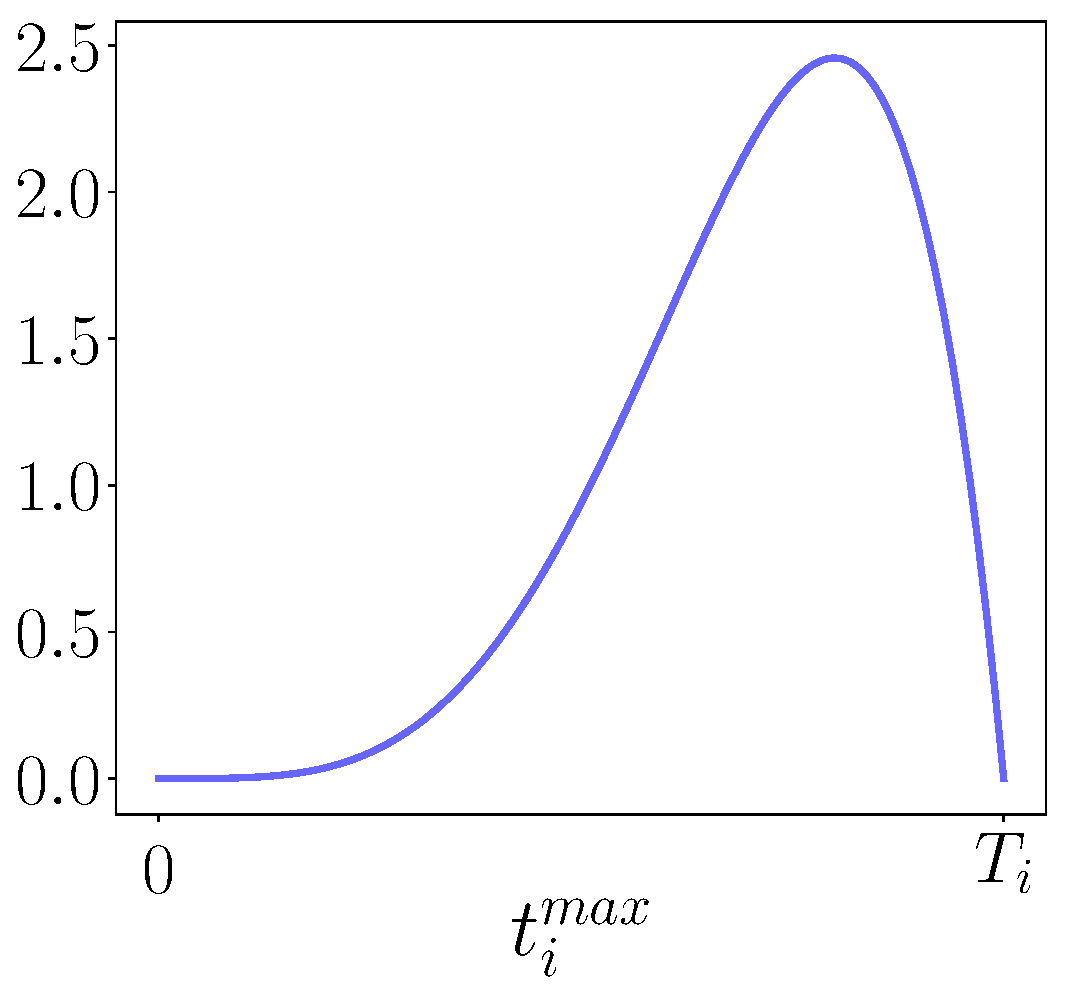
\includegraphics[width=.3\textwidth]{./figures/beta_law.pdf}
\label{fig:timax-pdf}}
\hspace{.02\textwidth}
\subfigure[exemple simu]{
% \includegraphics[width=.38\textwidth]{./figures/time2.pdf}
\label{fig:example-data}}
\caption{Illustrations of simulated data.}
\end{figure}

Following the real-time prediction paradigm presented in Section~\ref{sec:evaluation strategy}, we compare the predictive performances of the lights model with the competing ones introduced in Section~\ref{sec:competing models} in terms of C-index (see Section~\ref{sec:Metrics}).
We also want to assess the stability of the lights model in terms of feature selection, but we do not compare this aspect with state-of-the-art since other models are not designed to perform feature selection, and comparisons would be unfair. 
To this end, we follow the same simulation procedure explained in the previous lines and for each simulation case, we use the following approach to evaluate the variable selection power of the model. Denoting 
\[\tilde{\xi}_j = \dfrac{|\hat{\xi}_j|}{\max_{j=1,\ldots,p}{|\hat{\xi}_j|}} \qquad \text{and} \qquad \tilde{\gamma}_{k,a}^l = \dfrac{|\hat{\gamma}_{k,a}^l|}{\max_{a=1, \ldots, \cA}{|\hat{\gamma}_{k,a}^l|}}\] 
for $k=0,\ldots,K-1$ and $l=1, \ldots, L$, and considering that $\tilde{\xi}_j$ and $\tilde{\gamma}_{k,a}^l$ are the predicted probability that the true $\xi_j$ equals $\varsigma_1$ and the predicted probability that the true $\gamma_{k,a}^l$ equals $\varsigma_2$ respectively, then we are in a binary prediction setting and we use the two resulting AUC scores of this problem to evaluate the selection power of the time-independent and the time-dependent features respectively.

\subsection{Results of simulation}
\label{sec:simulation results}
Let us present now the simulation results.


\section{Applications}
\label{sec:application}

In this section, we apply our lights method on two publicly available datasets and compare its performance with state-of-the-art methods.

\subsection{The PBCseq dataset}

This dataset is a follow-up to the original dataset~\citep{fleming2011counting, murtaugh1994primary}from the Mayo Clinic trial in primary biliary cirrhosis (PBC) of the liver conducted between 1974 and 1984. 
A total of 424 PBC patients, referred to Mayo Clinic during that ten-year interval, met eligibility criteria for the randomized placebo controlled trial of the drug D-penicillamine. The first 312 cases in the data set participated in the randomized trial and contain largely complete data. The additional 112 cases did not participate in the clinical trial, but consented to have basic measurements recorded and to be followed for survival. Six of those cases were lost to follow-up shortly after diagnosis, so the data here are on an additional 106 cases as well as the 312 randomized participants. 
The dataset contains only baseline measurements of the laboratory paramters and contains multiple laboratory results, but only on the first 312 patients. 


\subsection{The MIMIC III dataset}

The MIMIC III (Medical Information Mart for Intensive Care III) database is a large, freely-available hospital dataset containing de-identified data from over 40,000 patients. This data comes from patients who were admitted in critical care units to Beth Israel Deaconess Medical Center in Boston, Massachusetts from 2001 to 2012~\citep{johnson2016mimic}. The dataset was populated with data that had been acquired during routine hospital care, so there was no associated burden on caregivers and no interference with their workflow.

% \url{https://www.nature.com/articles/sdata201635/}\\
% \url{https://ieeexplore.ieee.org/abstract/document/1166854}\\
% \url{https://www.sciencedirect.com/science/article/abs/pii/S2213260014702395}\\
% \url{https://www.sciencedirect.com/science/article/pii/S2352556818302169}\\
% }


\section{Conclusion}
\label{sec:conclusion}

In this paper, a generalized joint model for high-dimensional multivariate longitudinal data and censored durations (lights) has been introduced, and a new efficient estimation
algorithm (QNMCEM) has been derived, that considers a penalization of the likelihood in order to perform feature
selection and to prevent overfitting.


\section*{Software}
All the methodology discussed in this paper is implemented in \texttt{Python}. The code is available from \url{https://github.com/Califrais/lights} in the form of annotated programs, together with a notebook tutorial. A technical documentation is also provided in Appendix~\ref{sec:package}.

\section*{Acknowledgements}
\textit{Conflict of Interest}: None declared.

\appendix

\begin{center}
\LARGE \textbf{Appendices}
\end{center}

\section{Proof of Lemma~\ref{lemma:prox-sgl1}}
\label{sec:proof-lemma-prox-sgl1}



\section{Automatic cross-validation grid for $\xi$}
\label{sec:auto-grid-cv}

Concerning the cross-validation procedure for tuning 
\[(\zeta_{1,0}, \zeta_{2,0}, \zeta_{3,0}, \ldots, \zeta_{1,K-1}, \zeta_{2,K-1}, \zeta_{3,K-1})^\top \in \R_+^{3K}, \]
we use a randomized search with the C-index metric (see Section~\ref{sec:evaluation strategy}) where for all $k=0, \ldots, K-1$ and $j \in \{1, 2, 3\}$, each $\zeta_{j,k}$ finds its candidates in the interval 
\[[\zeta_{j,k}^{\text{max}} \times 10^{-4}, \zeta_{j,k}^{\text{max}} ] \subset \R, \]
with $\zeta_{j,k}^{\text{max}}$ the interval upper bound computed hereafter.

Considering the convex minimization problem~\eqref{eq:minimization-xi_k} at a given step $w$,
let us denote $\zeta_{1,k}^1 \leq \zeta_{1,k}^2 \leq \dots \leq \zeta_{1,k}^{\text{max}}$ the randomly chosen candidate values for $\zeta_{1,k}$, such that at $\zeta_{1,k}^{\text{max}}$, all coefficients $\hat \xi_{k, j}$ for all $j = 1, \dots, p$ are exactly zero.
The KKT conditions~\citep{boyd2004convex} claim that
\begin{center}
  $\left\{
      \begin{aligned}
        &\frac{\partial P_{n, k}^{(w)}(\hat \xi_k)}{\partial \xi_{k,j}} =  \zeta_{1,k} \big( (\eta-1)\ \text{sgn}(\hat \xi_{k,j}) - \eta \hat \xi_{k,j} \big)  \quad \ \ \ \forall j \in \hat \cA_k \\
        &\left| \frac{\partial P_{n, k}^{(w)}(\hat \xi_k)}{\partial \xi_{k,j}} \right| < \zeta_{1,k} (1 - \eta) \quad \quad \quad \quad \quad \quad \quad \ \forall j \notin \hat \cA_k
      \end{aligned}
    \right.$,
\end{center}
where $\hat \cA_k = \big\{j = 1, \dots, p : \hat \xi_{k,j} \neq 0 \big\}$ is the active set of the $\hat \xi_k $ estimator, and for all $x \in~\R\setminus~\{0\},\ \text{sgn}(x) = \mathds{1}_{\{x>0\}} - \mathds{1}_{\{x<0\}} $. Then, using~\eqref{eq:grad-xi_k}, one obtains
\begin{equation*}
\hat \xi_{k, j} = 0 \ \Rightarrow \ \left| n^{-1} \sum_{i=1}^n \hat \pi_{ik}^{\theta^{(w)}} \big( 1 - \pi_{\xi_k}(x_i) \big) x_{ij}  \right| < \zeta_{1,k} (1 - \eta)
\end{equation*}
for all $j = 1, \dots, p$.
Hence, we choose the following upper bound for the randomly chosen candidate interval during the cross-validation procedure
\begin{equation*}
\zeta_{1,k}^{\text{max}} = \frac{1}{n(1-\eta)} \underset{j = 1, \dots, p}{\text{max}} \sum_{i=1}^n |x_{ij}|.
\end{equation*}
Similar strategy to automatically compute $\zeta_{2,k}^{\text{max}}$ or $\zeta_{3,k}^{\text{max}}$ is not easy since without additionnal hypothesis, the gradients~\ref{eq:grad-beta_k},~\ref{eq:grad-Q-1} and~\ref{eq:grad-Q-2} are not upper bounded by a quantity that depends only on the data and not on the current iteration parameters estimates. We then choose those interval upper bounds empirically.

\section{Event time simulation}
\label{sec:event-time-simu}

Let us derive here the expression~\eqref{eq:time-generation} used to generate event times. Indeed, we can not refer to~\citet{austin2012generating} since the intensity~\eqref{eq:baseline} of the baseline is not correct in this paper.
Note that other errors had already been pointed in~\citep{austin2013correction}, for instance the fact that there is no closed-form expression with a Weibull baseline.
Suppose that
\[\lambda(t) = \lambda_0(t) \exp (a + b t)\]
with $(a, b) \in \R^2$ and $\lambda_0$ defined in~\eqref{eq:baseline}, then the cumulative hazard function writes
\[H(t) = \kappa_1 \kappa_2 e^a \int_0^t \exp\{(\kappa_2 + b)s \} \dd s = \dfrac{\kappa_1 \kappa_2 e^a}{\kappa_2 + b} \big( \exp\{(\kappa_2 + b) t\} - 1 \big).\]
Then, on has
\[t = \dfrac{1}{\kappa_2 + b} \log \Big( 1 + \dfrac{H(t)(\kappa_2 + b)}{\kappa_1 \kappa_2 e^a} \Big),\]
and one can generate event times according to
\[ T \sim \dfrac{1}{\kappa_2 + b} \log \Big( 1 - \dfrac{(\kappa_2 + b)\log U}{\kappa_1 \kappa_2 e^a} \Big) \]
with $U \sim \cU\big([0,1]\big)$.
$\hfill\square$

\section{Multivariate linear mixed model}
\label{sec:MLMM}

Let us derive here the explicit EM algorithm for the multivariate linear mixed model used to initialized the longitudinal parameters $\beta_k^{(0)}$, $D^{(0)}$ and $\phi^{(0)}$ in the QNMCEM algorithm in Section~\ref{sec:QNMCEM}, acting as if there is no subgroup ($\beta_0^{(0)} = \cdots = \beta_{K-1}^{(0)}$). 
For the sake of simplicity, let us denote here 
\[\theta = (\beta^\top, \text{vech}(D), \phi^\top)^\top \in \R^\vartheta\]
the parameter vector to infer.
The conditional distribution of $y_i|b_i$ then writes
\[f(y_i|b_i ; \theta) = \exp \big\{( \Sigma_iy_i)^\top M_{i} - c_\phi(M_{i}) + d_\phi(y_i) \big\},\]
where $\Sigma_i$ is the diagonal matrix whose diagonal is $\Phi_i$. 
The complete log-likelihood in this context writes
\begin{align*}
\ell_n^\text{comp}(\theta) &= \ell_n^\text{comp}(\theta ; \cD_n, \textbf{\textit{b}}) \\
&= \sum_{i=1}^n (\Sigma_iy_i)^\top M_{i} - c_\phi(M_{i}) + d_\phi(y_i) -\dfrac12 \big(r \log 2\pi + \log|D| + b_i^\top D^{-1}b_i\big).
\end{align*}
  
\paragraph*{E-step.}
Supposing that we are at step $w + 1$ of the algorithm, with current iterate denoted $\theta^{(w)}$, we need to compute the expected negative log-likelihood of the complete data conditional on the observed data and the current estimate of the parameters, which is given by 
\[\cQ_n(\theta, \theta^{(w)}) = \E_{\theta^{(w)}}[\ell_n^\text{comp}(\theta) | \cD_n].\]
Here, computing this quantity reduces to computing $\E_{\theta^{(w)}}[b_i | y_i]$ and $\E_{\theta^{(w)}}[b_ib_i^T | y_i]$ for $i = 1,\ldots,n$.
The marginal distributions of $y_i$ and $b_i$ being both Gaussian, one has from Bayes Theorem
\[ f(b_i|y_i; \theta^{(w)}) \propto \exp \big\{ -\dfrac12 (b_i - \mu_i^{(w)})^\top {\Omega_i^{(w)}}^{-1} (b_i - \mu_i^{(w)}) \big\}\]
where
\[\Omega_i^{(w)} = ({V_i}^\top \Sigma_i^{(w)}V_i + {D^{(w)}}^{-1})^{-1} \quad \text{ and } \quad \mu_i^{(w)} = \Omega_i^{(w)}{V_i}^\top \Sigma_i^{(w)}(y_i - U_i\beta^{(w)}).\]
Then, on has
\begin{center}
  $\left\{
    \begin{aligned}
      &\E_{\theta^{(w)}}[b_i | y_i] = \mu_i^{(w)}, \\
      &\E_{\theta^{(w)}}[b_ib_i^T | y_i] = \Omega_i^{(w)} + \mu_i^{(w)}{\mu_i^{(w)}}^\top.
    \end{aligned}
    \right.$
\end{center}

\paragraph*{M-step.}
Here, we need to compute \[\theta^{(w+1)} \in \argmin_{\theta \in \R^\vartheta} \cQ_n(\theta, \theta^{(w)}) .\]
The parameters updates are then naturally given in closed form by zeroing the gradient. One obtains
\[\beta^{(w+1)} = \Big(\sum_{i=1}^n U_{i}^\top U_{i}\Big)^{-1}  \sum_{i=1}^n \big[ U_{i}^\top  y_i - U_{i} V_{i} \E_{\theta^{(w)}}[ b_i | y_i]) \big],\]
\begin{align*}
\phi_l^{(w+1)} = \big(\sum_{i=1}^n n_i^l \big)^{-1}  \sum_{i=1}^n \Big[(&y_i^l - U_{il}\beta_l^{(w+1)})^\top (y_i^l - U_{il}\beta_l^{(w+1)} - 2V_{il}\E_{\theta^{(w)}}[b_i^l | y_i^l])) \\
&+\Tr\big(V_{il}^\top V_{il} \E_{\theta^{(w)}}[ b_i^l {b_i^l}^\top | y_i^l]\big) \Big]
\end{align*}
and \[D^{(w+1)} = n^{-1} \sum_{i=1}^n \E_{\theta^{(w)}}[ b_i {b_i}^\top | y_i].\]


\section{Technical documentation of the \texttt{lights} package}
\label{sec:package}

\subsection{\texttt{MLMM class}}

This class implements an EM algorithm for fitting a multivariate linear mixed model used to initialize the MCQNEM algorithm.
Let us introduce the list $\Omega^{(w)} = [\Omega_1^{(w)}, \ldots, \Omega_n^{(w)}]$, the matrices $\mu = [\mu_1, \ldots, \mu_n] \in \R^{r \times n}$, $U^l = [{U_{1l}}^\top \cdots {U_{nl}}^\top]^\top \in \R^{n_l \times q_l}$, $U = [U_1^\top \cdots U_n^\top]^\top \in \R^{\cN \times q}$,
\[ V^l = \begin{bmatrix}
    V_{1l} & \cdots & 0\\
    \vdots &  \ddots & \vdots \\
    0 & \cdots & V_{nl}
\end{bmatrix},
\quad
V = \begin{bmatrix}
  V_{1} & \cdots & 0\\
  \vdots &  \ddots & \vdots \\
  0 & \cdots & V_{n}
\end{bmatrix}
\quad \text{ and } \quad
{\Omega^l}^{(w)} = \begin{bmatrix}
    {\Omega_{1}^l}^{(w)} & \cdots & 0\\
    \vdots &  \ddots & \vdots \\
    0 & \cdots & {\Omega_{n}^l}^{(w)}
\end{bmatrix}\]
that belong respectively in $\R^{n_l \times nr_l}$, $\R^{\cN \times nr}$ and $\R^{nr_l \times nr_l}$, as well as the vectors $\tilde \mu^{(w)} = ({\mu_1^{(w)}}^\top \cdots {\mu_n^\top)^{(w)}}^\top \in \R^{nr}$, $(\tilde \mu^l)^{(w)} = \big({(\mu_1^l)^{(w)}}^\top \cdots {(\mu_n^l)^{(w)}}^\top \big)^\top \in \R^{nr_l}$, $y^l = ({y_1^l}^\top  \cdots {y_n^l}^\top)^\top \in \R^{n_l}$
with $n_l = \sum_{i=1}^{n} n_i^l$ and $y = (y_1^\top \cdots y_n^\top)^\top \in \R^\cN$ with $\cN = \sum_{i=1}^{n} n_i$.
The $\beta$ update then rewrites
\[\beta^{(w+1)} = ({U}^\top U)^{-1}{U}^\top(y-V \tilde \mu^{(w)}).\]
For the $D$ update, one has
\[D^{(w+1)} = n^{-1} \big( \text{sum}(\Omega^{(w)}) + \mu^{(w)}{\mu^{(w)}}^\top\big).\]
And finally for the $\phi$ update, one has
\begin{align*}
\phi_l^{(w+1)} = n_l^{-1} \big[&(y^l - U^l{\beta_l^{(w+1)})}^\top \big(y^l - U^l\beta_l^{(w+1)} - 2 V^l (\tilde\mu^l)^{(w)}\big) \\
&+ \text{Tr}\big\{{V^l}^\top V^l \big({\Omega^l}^{(w)} + (\tilde\mu^l)^{(w)} {(\tilde\mu^l)^{(w)}}^\top\big)\big\} \big].
\end{align*}

\bibliography{biblio}
\bibliographystyle{plainnat}{}
\end{document}
